\documentclass[APA,STIX1COL]{WileyNJD-v2}
\usepackage{siunitx}
\usepackage{graphicx}
\usepackage{subcaption}
\usepackage{float}        % for [H] placement

\articletype{Research Article} % Specify article type

\received{Date Month Year}
\revised{Date Month Year}
\accepted{Date Month Year}
\copyyear{2025}
\startpage{1}

\raggedbottom

%%%%%%%%%%%%%%%%%%%%%%%%%%%%%%
% My commands:
\newcommand{\bruno}[1]{\textcolor{blue}{#1}} % Bruno Sanso edits - blue
\newcommand*\mymin[1][]{\min_{#1}\,}
\newcommand{\vect}[1]{\mathbf{#1}}  
\newcommand\numberthis{\addtocounter{equation}{1}\tag{\theequation}}
\newcommand\independent{\protect\mathpalette{\protect\independenT}{\perp}}
\def\independenT#1#2{\mathrel{\rlap{$#1#2$}\mkern2mu{#1#2}}}
%%%%%%%%%%%%%%%%%%%%%%%%%%%%%%

\begin{document}

\title{Bayesian Quantile-Based Correction and Synthesis of River Flow Forecasts\protect\thanks{This research was conducted as part of the PhD dissertation of the first author at the University of California, Santa Cruz.}}

\author[1]{Antonio Aguirre*}
\author[1]{Raquel Prado}
\author[1]{Bruno Sans\'o}

\authormark{Aguirre \textsc{et al.}} % Running head author name

\address[1]{\orgdiv{Department of Statistics}, \orgname{University of California, Santa Cruz}, \orgaddress{\state{California}, \country{USA}}}

\corres{*Corresponding author: Antonio Aguirre. \email{jaguir@ucsc.edu}}

\presentaddress{University of California, Santa Cruz, Santa Cruz, CA, USA.}

\abstract[Summary]{River-flow forecasting requires predictive distributions that remain informative in both routine and extreme conditions. We develop a Bayesian quantile-based correction-and-synthesis framework built on Dynamic Quantile Linear Models (DQLMs). The framework links USGS observations, retrospective products, and ensemble forecast products through a shared latent quantile process, learns dynamic discrepancies for each external source, and combines quantile-specific posterior predictions into a single predictive distribution. We also adapt variational Bayes inference to the extended dynamic quantile linear model using Laplace--Delta approximations for non-conjugate parameters. The methodology is studied using daily flow for the San Lorenzo River together with ECMWF/GloFAS and NOAA/NWS products, with emphasis on medium-range forecasting and uncertainty quantification across multiple quantile levels.}

\keywords{Bayesian forecasting, quantile regression, dynamic models, river flow prediction}

\jnlcitation{\cname{%
\author{Aguirre A.}, 
\author{Prado R.}, and 
\author{Sans\'o B.}} (\cyear{2025}), 
\ctitle{Bayesian quantile-based correction and synthesis of river flow forecasts}, \cjournal{Environmetrics}, \cvol{XX:1--20}.}

\maketitle

\footnotetext{\textbf{Abbreviations:} CRPS, Continuous Ranked Probability Score; DQLM, Dynamic Quantile Linear Model.}


\section{INTRODUCTION}

River flow forecasts are used for flood preparedness, drought monitoring, reservoir operations, and water-supply planning. In settings such as Santa Cruz, California, forecast quality depends both on hydrological modeling of river response and on the quality of meteorological inputs that drive that response. These two uncertainty sources are related but distinct. Hydrological uncertainty arises from model structure, parameters, states, and observations within the river system, whereas meteorological uncertainty enters through imperfect precipitation and related atmospheric forcing fields \citep{tarek2021daily, thiboult2016accounting, kim2019hybrid, haiden2021evaluation}. A useful statistical forecasting framework should keep these roles clear while still allowing them to interact in the final predictive distribution.

Operational hydrological forecasts are commonly produced with conceptual or physically based models and are increasingly distributed as ensemble products. Those products are useful, but they often differ in horizon, spatial resolution, assimilation strategy, and uncertainty representation \citep{molteni1996ecmwf, isaksen2010ensemble, demargne2013science, barlage2021importance, johnson2023comprehensive}. Retrospective products introduce a different source of information: they provide historically consistent reconstructions that can be compared against observations to learn systematic discrepancies. The statistical problem addressed here is how to combine observations, retrospective products, and forecast products in a way that improves predictive distributions for river flow.

This problem is closely related to forecast combination and statistical post-processing, where multiple predictive sources are combined to improve calibration and sharpness \citep{siegert2019forecast, vannitsem, wang2022forecastcombinations50yearreview}. Bayesian formulations are especially appealing because they provide a coherent way to propagate uncertainty and update predictions as new information becomes available \citep{duan2006bma, yumnam2022quantile, aastveit2022quantifying, du2018ensemble_forecasting, doubleday, kleiber2011geostatistical, mcalinn2019dynamic, tallman2023bayesianpredictivedecisionsynthesis, johnson2023bayesian}. Our focus is on a quantile-based version of this problem, motivated by the need to represent both routine and extreme flow behavior.

We develop a Bayesian quantile-based correction-and-synthesis framework for river flow forecasts. The framework builds on Dynamic Quantile Linear Models (DQLMs) \citep{goncalves, gourieroux2008dqlm, barata2021_flex_quantile} and has three main components. First, we extend posterior inference for the model using scalable variational Bayes methods for the extended dynamic quantile linear model, following the Laplace--Delta strategy of \citet{wang2013nonconjugatevb}. Second, we use retrospective products to learn dynamic discrepancies relative to USGS observations and propagate those discrepancies into the forecast period. Third, we synthesize the resulting quantile-specific predictive distributions into one predictive distribution for the river flow process.

We study this framework using daily river flow for the San Lorenzo River together with retrospective and forecast products from ECMWF/GloFAS and NOAA/NWS. The empirical focus is forecasting performance and uncertainty quantification across multiple quantile levels, rather than only historical fit or methodological development in isolation. Although the application is hydrological, the same structure is relevant in other settings where observations, retrospective products, and forecast products all play distinct roles.

The remainder of the paper is organized as follows. Section~\ref{sec:methodology} presents the modeling framework and inference strategy. Section~\ref{sec:data} describes the San Lorenzo application, the data sources, and the rolling-origin forecasting design. Section~\ref{sec:forecastvalidation} reports the out-of-sample forecast validation results, and Section~\ref{sec:interpretation} presents supporting interpretation for the selected specification. Section~\ref{sec5} concludes.

\section{METHODOLOGY}
\label{sec:methodology}

We first introduce some notation to be used throughout the article. We use bold uppercase letters (e.g., $\mathbf{W}, \mathbf{F}, \mathbf{G}$) to denote matrices, and bold lowercase letters (e.g., $\mathbf{x}, \mathbf{\psi}, \mathbf{\theta}$) to denote vectors. We denote the identity matrix of dimension $m \times m$ as $\mathbf{I}_m$, a vector of zeros of dimension $m \times 1$ as $\mathbf{0}_m$, and a vector of ones of dimension $m \times 1$ as $\mathbf{1}_m$.

\subsection{Flexible Quantile Estimation: The Extended Asymmetric Laplace}
\label{subsec:exal}

The use of the Asymmetric Laplace (AL) distribution for quantile inference within a Bayesian framework is well-established with both empirical and theoretical justifications \citep{yu2001bayesian, sriram2013theoretical}. We use a recent extension of the AL distribution, which we refer to as the extended asymmetric Laplace (exAL), that addresses intrinsic issues for the AL working likelihood, such as the limitations imposed by its skewness. \citet{yan2025new} proposed the extended asymmetric Laplace (exAL) distribution, $\text{exAL}_{p_0}(\mu, \sigma, \gamma)$, where $\mu$ represents the $p_0$th quantile of interest, $\sigma$ is a positive scale parameter, and $\gamma$ is the skewness parameter. Moreover, the parameter $\gamma$ has bounded support over the interval $(L, U)$, where $L$ is the negative root of $g(\gamma) = 1 - p_0$ and $U$ is the positive root of $g(\gamma) = p_0$, with $g(\gamma) = 2 \Phi(-|\gamma|) \exp(\gamma^2 / 2)$ and $\Phi$ denoting the standard normal CDF. To improve the efficiency of our posterior sampling algorithms, we utilize the extended stochastic representation of an exAL random variable described in \citet{yan2025new}. That is, if $y \sim \text{exAL}(\mu, \sigma, \gamma)$, then there exist independent random variables $\epsilon \sim \mathcal{N}(0, 1)$, $z \sim \text{Exp}(1)$, and $s \sim \mathcal{N}^+(0, 1)$, (where $\mathcal{N}^+(0, 1)$ denotes the standard normal distribution truncated to the positive real line), such that  \( y = \mu + C(\gamma; p_0)\sigma |\gamma| s + A(\gamma; p_0) \sigma z + \sqrt{B(\gamma; p_0) \sigma^2 z} \cdot \epsilon, \) where $A(\gamma; p_0) = \frac{1 - 2 p(\gamma; p_0)}{p(\gamma; p_0) \, [1 - p(\gamma; p_0)]}$, $B(\gamma; p_0) = \frac{2}{p(\gamma; p_0) \, [1 - p(\gamma; p_0)]}$, $C(\gamma; p_0) = [I(\gamma > 0) - p(\gamma; p_0)]^{-1}$, and $p(\gamma; p_0) = I(\gamma < 0) + \{p_0 - I(\gamma < 0)\} / g(\gamma)$.


\subsection{Unified State-Space Model}
\label{subsec:fullmodel}

We write the forecasting framework directly as one state-space model. The same latent state is used throughout the estimation period and the forecast window; what changes after the cutoff is the set of observation channels that remains available, together with the forecast-window covariance specification used to propagate the state. Let
\[
\boldsymbol{\eta}_t =
\begin{bmatrix}
\boldsymbol{\theta}_t \\
\boldsymbol{\delta}_t^1 \\
\vdots \\
\boldsymbol{\delta}_t^J \\
\zeta_t \\
\boldsymbol{\psi}_t
\end{bmatrix},
\]
where \(\boldsymbol{\theta}_t \in \mathbb{R}^p\) contains the trend and seasonal states, \(\boldsymbol{\delta}_t^j \in \mathbb{R}^p\) is the discrepancy state for source \(j\), \(\zeta_t \in \mathbb{R}\) is the transfer state, and \(\boldsymbol{\psi}_t \in \mathbb{R}^m\) contains the time-varying covariate effects. The transfer block evolves through
\[
\mathbf{G}^{\text{trans}}_t =
\begin{bmatrix}
\lambda & \mathbf{x}_t' \\
\mathbf{0}_m & \mathbf{I}_m
\end{bmatrix},
\]
with \(\lambda\) governing persistence in the transfer state and \(\mathbf{x}_t\) denoting the external covariates.

Using this notation, the full T1 specification can be written line by line as follows:
\begin{align}
\text{USGS observations:}&&
y_t^o \mid \boldsymbol{\eta}_t, \sigma^o, \gamma^o
&\sim \text{exAL}_{p_0}\!\left(\mathbf{F}_t' \boldsymbol{\theta}_t + \zeta_t, \sigma^o, \gamma^o\right),
\quad 1 \le t \le T, \label{eq:unified_usgs}
\\
\text{Retrospective products:}&&
z_t^j \mid \boldsymbol{\eta}_t, \sigma^j, \gamma^j
&\sim \text{exAL}_{p_0}\!\left(\mathbf{F}_t'(\boldsymbol{\theta}_t + \boldsymbol{\delta}_t^j) + \zeta_t, \sigma^j, \gamma^j\right),
\quad 1 \le j \le J,\ 1 \le t \le T, \label{eq:unified_retro}
\\
\text{Forecast products:}&&
y_T^{j,i}(k) \mid \boldsymbol{\eta}_{T+k}, \sigma^j, \gamma^j
&\sim \text{exAL}_{p_0}\!\left(\mathbf{F}_{T+k}'(\boldsymbol{\theta}_{T+k} + \boldsymbol{\delta}_{T+k}^j) + \zeta_{T+k}, \sigma^j, \gamma^j\right), \nonumber\\
&&&
\qquad 1 \le j \le J,\ 1 \le i \le I_j,\ 1 \le k \le K_{(j)}, \label{eq:unified_forecast}
\\
\text{Trend and seasonal states:}&&
\boldsymbol{\theta}_t \mid \boldsymbol{\theta}_{t-1}
&\sim \mathcal{N}\!\left(\mathbf{G}_t \boldsymbol{\theta}_{t-1}, \mathbf{W}_t^\theta\right), \label{eq:unified_theta}
\\
\text{Discrepancy states:}&&
\boldsymbol{\delta}_t^j \mid \boldsymbol{\delta}_{t-1}^j
&\sim \mathcal{N}\!\left(\mathbf{G}_t \boldsymbol{\delta}_{t-1}^j, \mathbf{W}_t^{\delta^j}\right),
\quad 1 \le j \le J, \label{eq:unified_delta}
\\
\text{Transfer-function states:}&&
\begin{bmatrix}
\zeta_t \\
\boldsymbol{\psi}_t
\end{bmatrix}
\Bigg|
\begin{bmatrix}
\zeta_{t-1} \\
\boldsymbol{\psi}_{t-1}
\end{bmatrix}
&\sim \mathcal{N}\!\left(
\mathbf{G}^{\text{trans}}_t
\begin{bmatrix}
\zeta_{t-1} \\
\boldsymbol{\psi}_{t-1}
\end{bmatrix},
\text{BlockDiag}\!\left(w_t^\zeta, \mathbf{W}_t^\psi\right)
\right). \label{eq:unified_transfer}
\end{align}

The source-specific parameters are \((\sigma^o,\gamma^o)\) for the USGS series and \((\sigma^j,\gamma^j)\) for all channels associated with source \(j\), whether retrospective or forecast-based. Here \(T\) denotes the cutoff or forecast origin, so \(y_T^{j,i}(k)\) is the \(k\)-step-ahead member issued at that origin. The first two lines describe the estimation period, where the available observations are the USGS series and the retrospective products. The third line describes the forecast window, where those channels are replaced by the forecast products issued at or before the cutoff. The same state components persist throughout, so the forecast window is treated as a continuation of the same latent process rather than as a separate model. In the T1 specification, the transfer block remains active after the cutoff, with \(\mathbf{x}_t\) given by the forecast covariates available at that origin. The T0 benchmark used in Section~\ref{subsec:benchmarkresults} is obtained by suppressing the forecast-window transfer block after the cutoff.

For later reference, the same model can be written in compact form. During the estimation period,
\begin{align}
y_{t,s} \mid \boldsymbol{\eta}_t, \sigma_s, \gamma_s
&\sim \text{exAL}_{p_0}\!\left(\mathbf{h}_{t,s}' \boldsymbol{\eta}_t, \sigma_s, \gamma_s\right),
\quad s \in \{0,1,\ldots,J\}, \label{eq:compact_est_obs}
\\
\boldsymbol{\eta}_t \mid \boldsymbol{\eta}_{t-1}
&\sim \mathcal{N}\!\left(\boldsymbol{D}_t \boldsymbol{\eta}_{t-1}, \boldsymbol{\Lambda}_t\right),
\qquad 1 \le t \le T, \label{eq:compact_est_state}
\end{align}
where
\[
\mathbf{h}_{t,0} =
\begin{bmatrix}
\mathbf{F}_t \\
\mathbf{0}_{pJ} \\
1 \\
\mathbf{0}_m
\end{bmatrix},
\qquad
\mathbf{h}_{t,j} =
\begin{bmatrix}
\mathbf{F}_t \\
\mathbf{0}_{p(j-1)} \\
\mathbf{F}_t \\
\mathbf{0}_{p(J-j)} \\
1 \\
\mathbf{0}_m
\end{bmatrix},
\quad 1 \le j \le J,
\]
and
\[
\boldsymbol{D}_t = \text{BlockDiag}\!\left(\mathbf{G}_t, \mathbf{G}_t, \ldots, \mathbf{G}_t, \mathbf{G}^{\text{trans}}_t\right), \qquad
\boldsymbol{\Lambda}_t = \text{BlockDiag}\!\left(\mathbf{W}^{\theta}_t, \mathbf{W}^{\delta^1}_t, \ldots, \mathbf{W}^{\delta^J}_t, w_t^{\zeta}, \mathbf{W}^{\psi}_t\right).
\]
Thus, \(\mathbf{h}_{t,0}' \boldsymbol{\eta}_t = \mathbf{F}_t' \boldsymbol{\theta}_t + \zeta_t\) and \(\mathbf{h}_{t,j}' \boldsymbol{\eta}_t = \mathbf{F}_t'(\boldsymbol{\theta}_t + \boldsymbol{\delta}_t^j) + \zeta_t\).

During the forecast window,
\begin{align}
y_{t,(j,i)} \mid \boldsymbol{\eta}_t, \sigma^j, \gamma^j
&\sim \text{exAL}_{p_0}\!\left(\mathbf{e}_{t,j}' \boldsymbol{\eta}_t, \sigma^j, \gamma^j\right),
\quad 1 \le j \le J,\ 1 \le i \le I_j,\ t-T \le K_{(j)}, \label{eq:compact_fc_obs}
\\
\boldsymbol{\eta}_t \mid \boldsymbol{\eta}_{t-1}
&\sim \mathcal{N}\!\left(\boldsymbol{M}_t \boldsymbol{\eta}_{t-1}, \mathbf{W}_t\right),
\qquad T < t \le T + K_{(1)}. \label{eq:compact_fc_state}
\end{align}
Here \(\mathbf{e}_{t,j}\) is the forecast-window analogue of \(\mathbf{h}_{t,j}\): it extracts the latent trend-and-seasonal block, the discrepancy block for source \(j\), and, in the T1 specification, the transfer block. The matrix \(\boldsymbol{M}_t\) preserves the same block structure as \(\boldsymbol{D}_t\) while propagating the state through the forecast window. In computation, we use reduced forecast-window matrices that retain only the forecasters whose horizons remain active at each lead time; this reduction is computational only and does not change the underlying model.

This single formulation recovers the earlier Models A, B, and C as restrictions. Model A is obtained by suppressing the discrepancy states and retaining only the USGS observation channel. Model B is obtained by keeping the USGS and retrospective channels but restricting attention to \(1 \le t \le T\). Model C is the full specification in \eqref{eq:unified_usgs}--\eqref{eq:compact_fc_state}, where the same latent state is continued into the forecast window and the active observation channels change after the cutoff.

\subsection{Prior Specification and Discount Factors}
\label{subsec:prioranddisc}
Following \citet{barata2021_flex_quantile}, for each skewness parameter, we assign a truncated Student-t prior: \(\gamma^j \sim t_{(L, U)}(0, \phi^j, \nu^j)\), where $\phi^j$ and $\nu^j$ denote the scale and degrees of freedom hyperparameters, respectively, for \(1 \leq j \leq J\). For the scale parameters, we use inverse gamma priors: \(\sigma^j \sim IG(a_{\sigma^j}, b_{\sigma^j})\), with $a_{\sigma^j}$ and $b_{\sigma^j}$ as shape and scale hyperparameters. The latent trend-and-seasonal block is initialized as \(\boldsymbol{\theta}_0 \sim \mathcal{N}(\mathbf{m}_0, \mathbf{C}_0)\), with $\mathbf{m}_0$ and $\mathbf{C}_0$ as location and scale hyperparameters.

Discount factors \citep{prado2021time} are used for adaptive evolution of the covariance matrices at the state level. Discount factors lie in the $(0,1]$ range, with 1 indicating no dynamic evolution and smaller values implying greater temporal adaptability. We use component discounting. The application-specific choices are given in Subsection~\ref{subsec:specification}. During the forecasting period ($t \in \{T+1, \ldots, T+K\}$), we set the Inverse Wishart prior parameters as $\mathbf{S}_t = (\nu_t - p_t - 1)\, c\, \mathbf{W}_T$ and $\nu_t = (p_t + 1 + \epsilon)$, with $\epsilon, c > 0$. Under this specification, the posterior mean is
\(
\mathbb{E}[\mathbf{W}_t \mid \mathcal{D}_t] = \frac{\epsilon}{1 + \epsilon}(c\, \mathbf{W}_T) + \frac{1}{1 + \epsilon} \mathbb{E}\left[ (\boldsymbol{\eta}_t - \mathbf{M}_t \boldsymbol{\eta}_{t-1}) (\boldsymbol{\eta}_t - \mathbf{M}_t \boldsymbol{\eta}_{t-1})' \mid \mathcal{D}_t \right],
\)
where $\mathcal{D}_t$ denotes all data available up to and including time $t$.

This specification yields a convex combination between a scaled version of the last covariance learned from observed data, $\mathbf{W}_T$, and the empirical residual covariance at time $t$. We set $\nu_t = p_t + 1 + \epsilon$ with $\epsilon = T$ to reflect the effective prior sample size contributed by the full estimation period. This stabilizes $\mathbf{W}_{T+k}$ over the short forecast horizon and avoids noisy covariance estimates. The scalar \(c\) inflates the prior covariance \(\mathbf{W}_T\); we set \(c = 10^2\) to avoid overconfidence when extrapolating the estimation-period covariance into the forecast window and to allow enough flexibility when forecast-period signals differ from the pre-cutoff regime. In a brief sensitivity check (\(c \in \{1,5^2,10^2,20^2\}\)), \(c=10^2\) provided the best balance.
 
Further details regarding prior specification and discount factors are provided in Subsection~\ref{subsec:specification}.

\subsection{Posterior Inference}
\label{subsec:postinf}
The posterior distribution of all model parameters is explored using a Markov chain Monte Carlo (MCMC) algorithm.
Algorithm~\ref{alg1} gives the core MCMC updates in a compact source-indexed notation. During the estimation period, the active source channels are the USGS observations and retrospective products; after the cutoff, the same updates use the active forecast-product channels, with additional bookkeeping for the reduced forecast-window matrices when forecast horizons differ across agencies. All full conditional posteriors are available in closed form except for the skewness parameters $\gamma^j$, $1 \leq j \leq J$. For these, we use a Metropolis--Hastings random walk on an unconstrained reparameterization. Posterior sampling of the state parameters relies on a modified Forward Filtering Backward Sampling (FFBS) algorithm that leverages their conditional normality (see Algorithm~\ref{alg:Alg2}).

%\subsubsection{Variational Bayes Implementation} \label{subsec:vb}

Given the computational demands of traditional Markov Chain Monte Carlo (MCMC) methods on large datasets, we also implement a Mean Field Variational Bayes (MFVB) algorithm to approximate posterior inference.
\citet{barata2021_flex_quantile} proposed a Variational Bayes algorithm that embeds an importance sampling scheme for non-conjugate parameters; however, this scheme risks particle collapse in high dimensions and requires further constraints to avoid degeneracy. In particular, it fixes the scale parameter of the exAL using pre-estimated values from an AL model. 
Building on \citet{barata2021_flex_quantile}, we address stability issues in their importance sampling approach by adopting the Variational Bayes Laplace-Delta (VB-LD) methodology from \citet{wang2013nonconjugatevb}. This framework replaces the importance sampling strategy to handle non-conjugate parameters with a dual strategy: Laplace approximations for non-conjugate parameters and the use of the Delta method for computing expectations of functionals of the non-conjugate parameters.

To illustrate our VB-LD strategy, consider a generic joint distribution \( p(D,\boldsymbol{\eta}, \boldsymbol{\psi}) \) where $D$ denotes the data, \( \boldsymbol{\psi} \) denotes conjugate parameters and \( \boldsymbol{\eta} \) represents non-conjugate parameters. We employ a Mean Field Variational Bayes (MFVB) approximation, assuming a factorized posterior \( q(\boldsymbol{\eta})q(\boldsymbol{\psi}) \), and optimize these approximations via Coordinate Ascent Variational Inference (CAVI). The CAVI framework in this setting iteratively updates two components: the conjugate parameters \( \boldsymbol{\psi} \) through \( q(\boldsymbol{\psi}) \propto \exp\left(\mathbb{E}_{q(\boldsymbol{\eta})}[\log p(D, \boldsymbol{\eta}, \boldsymbol{\psi})]\right) \), which admits closed-form solutions, and the non-conjugate parameters \( \boldsymbol{\eta} \) via \( q(\boldsymbol{\eta}) \propto \exp(\ell(\boldsymbol{\eta})) \), where \( \ell(\boldsymbol{\eta}) = \mathbb{E}_{q(\boldsymbol{\psi})}[\log p(D, \boldsymbol{\eta}, \boldsymbol{\psi})] \). The latter update is intractable due to its non-analytic normalizing constant, which we address through two steps. First, a Laplace approximation constructs a Gaussian surrogate \( q(\boldsymbol{\eta}) \approx \mathcal{N}(\hat{\boldsymbol{\eta}}, \Sigma) \), where \( \hat{\boldsymbol{\eta}} = \arg\max_{\boldsymbol{\eta}} \ell(\boldsymbol{\eta}) \) and \( \Sigma = -\left[\nabla^2 \ell(\hat{\boldsymbol{\eta}})\right]^{-1} \), matching the mode and curvature of \( \ell(\boldsymbol{\eta}) \). Second, expectations \( \mathbb{E}_{q(\boldsymbol{\eta})}[g(\boldsymbol{\eta})] \) required for updating \( \boldsymbol{\psi} \) are approximated via a second-order Taylor expansion (Delta Method): \( \mathbb{E}[g(\boldsymbol{\eta})] \approx g(\hat{\boldsymbol{\eta}}) + \frac{1}{2}\text{Tr}\left[\nabla^2 g(\hat{\boldsymbol{\eta}}) \Sigma\right] \), propagating uncertainty through \( \Sigma \) without stochastic sampling. The VB-LD algorithm iterates between Laplace mode-finding (e.g., via Newton-Raphson) and conjugate updates using these Delta-approximated moments until the measured Evidence Lower Bound (ELBO) converges.

We present the pseudocode for the VB algorithm associated with our model in Algorithm~\ref{alg:Alg3} and Algorithm~\ref{alg:Alg4}.

\subsection{Model Selection}
\label{subsec:modelselection}

For model selection, we use the Continuous Ranked Probability Score (CRPS) rather than PIT-based diagnostics. Following \citet{barata2021_flex_quantile}, we treat the discount-factor specification as fixed within a candidate model and select the transfer rate \(\lambda\) by minimizing the average one-step-ahead CRPS. In particular,
\[
\lambda^{\text{opt}} \in \arg\min_{\lambda} \frac{1}{T}\sum_{t=1}^T \text{CRPS}(y_t,p_t^{\lambda}),
\]
where \(p_t^{\lambda}\) denotes the predictive distribution at time \(t\) under transfer rate \(\lambda\).

We use CRPS because it scores the full predictive distribution and accounts jointly for calibration and sharpness. For a predictive distribution \(\mathbf{G}\) and an observation \(y\), the CRPS is
\[
\text{CRPS}(y, \mathbf{G}) = \mathbb{E}_{Y \sim \mathbf{G}}|Y - y| - \frac{1}{2}\mathbb{E}_{Y,Y'\sim \mathbf{G}}|Y - Y'|.
\]
It also reduces to the mean absolute error for deterministic forecasts, which makes it a natural criterion for comparing the candidate predictive specifications considered below.

\section{APPLICATION DATA AND FORECASTING DESIGN}
\label{sec:data}

\subsection{Study Setting and Target Observations}

Our target series is the average daily natural water flow (in cubic feet per second) of the San Lorenzo River at the Big Trees USGS gauging station in Santa Cruz, California. The Big Trees location is characterized by minimal human intervention, so the recorded flow closely reflects natural river dynamics. The dataset covers May 29, 1987, through December 25, 2022, and contains 12,986 daily USGS observations (Figure~\ref{fig:sanlorenzo}).

The San Lorenzo River is a major water resource for the Santa Cruz area and is relevant to both flood response and longer-term water-supply planning. The record includes major flood episodes as well as prolonged dry conditions, so it supports analysis of both low-flow and high-flow behavior. Lower quantiles are therefore relevant for drought conditions, whereas upper quantiles are relevant for flood risk.

\begin{figure}[h]
\centering
\includegraphics[width=450pt]{DISC/usgs.png}
\caption{
Daily water flow (log-log scale, cm$^3$/s) of the San Lorenzo River at the Big Trees USGS station from May 29, 1987, to December 25, 2022. Observed daily flow (green) is displayed on the $\log(\log(x+1))$ scale. Vertical dashed lines and numbered labels indicate major flood-related events: (1) February 1998 flood, (2) levee and floodwall reconstruction (2004), (3) February 2017 flood, and (4) January 2023 flood. Horizontal dashed lines represent NOAA-defined minor (16.5 ft, 503 cm) and major (21.76 ft, 663 cm) flooding thresholds, both converted to the log-log scale.
}
\label{fig:sanlorenzo}
\end{figure}

The application combines the USGS target series with three additional information sources: forecast covariates, retrospective products, and forecast products. Each source plays a different role. The covariates enter the transfer component of the latent process, the retrospective products are used to learn source-specific discrepancies during the estimation period, and the forecast products are used to generate the post-cutoff predictive distributions.

\subsection{External Data Sources and Forecast Covariates}

The transfer component uses both local hydrological covariates and a large-scale climate factor. The local covariates are precipitation from the PRISM Climate Group \citep{prism} and soil moisture from ECMWF ERA5-Land \citep{ecmwf}. The ERA5-Land fields are reanalysis-based inputs rather than direct observations, and some variables may include short forecast components.

To represent broader climate conditions, we also use a collection of monthly climate and environmental indices from \citet{noaa_climate_indices}, including solar flux, Niño 1+2, the Oceanic Niño Index (ONI), the Southern Oscillation Index (SOI), the Western Hemisphere Warm Pool (WHWP), the Global Mean Temperature (GMT), the Northern Oscillation Index (NOI), the Atlantic Multidecadal Oscillation (AMO), and the Tropical South (TSA) and North Atlantic (TNA) indices. These series are interpolated to daily resolution to align with the hydrological data.

We summarize these climate indices with the first generalized dynamic principal component (GDPC) \citep{JSSv092c02}. The number of leads and lags is selected by leave-one-out cross-validation, and the first component explains 53.42\% of the total variability among the indices.

The transfer covariates used in the application are therefore standardized precipitation, standardized soil moisture, and the first GDPC factor. Figure~\ref{fig:covariates} shows these three explanatory series.

\begin{figure*}[hbt!]
\centering
\centerline{\includegraphics[width=450pt]{DISC/precip_soilmoisture_climatePC1_faceted_labeled.png}}
\caption{
Scaled daily series of local precipitation, local soil moisture estimates, and the first principal component derived from multiple climate and environmental indices. All series have been standardized for comparability.
}
\label{fig:covariates}
\end{figure*}

The external product families come from two agencies: the Global Flood Awareness System (GloFAS) operated by ECMWF, and the National Weather Service (NWS) operated by NOAA. Each agency contributes both a retrospective product and an operational forecast product.

The retrospective products enter the estimation period and are used to learn source-specific discrepancies relative to the USGS target series. Figure~\ref{fig:retrospectives} shows the corresponding retrospective series at the Big Trees station.

The operational forecast products are used only after a cutoff date. The NWS ensemble has 7 members: 6 members provide medium-range forecasts up to 8.5 days, and one control member extends to 10 days. The GloFAS ensemble contains 51 members, all providing medium-range forecasts for up to 28 days.

\begin{figure*}[hbt!]
\centering
\centerline{\includegraphics[width=450pt]{DISC/retrospective_log_discharge_plot_faceted.png}}
\caption{Retrospective analyses from NWS and GloFAS at the San Lorenzo Big Trees USGS Station.}
\label{fig:retrospectives}
\end{figure*}

\subsection{Application-Specific State Specification}
\label{subsec:specification}

For the San Lorenzo application, the shared latent quantile process combines a local level, three seasonal harmonics, and the transfer component defined in Section~\ref{sec:methodology}. The discrepancy states use the same dynamic backbone as the latent trend-and-seasonal block through the repeated \(\mathbf{G}_t\) blocks in the full state evolution. We first specify the trend and seasonal structure. The matrix \(\mathbf{G}_t\) is composed of a trend component and a seasonal component. For the trend component, we include a constant term to represent the long-term average level of the quantile of interest. This component is defined by the evolution matrix and observational vector:
\( \mathbf{G}^{\text{trend}}_t = [1], \quad
\mathbf{F}^{\text{trend}}_t = [1]. \) The seasonal component incorporates three harmonics identified through exploratory spectral analysis to capture various seasonal cycles: an annual harmonic (12 months), a semiannual harmonic (6 months), and a long-term harmonic with an approximately 81-month (6.8 years) cycle. The seasonal component's evolution matrix and observational vector are defined as:
\( \mathbf{G}^{\text{seas}}_t = \text{BlockDiag}\left(\textbf{J}_2(1,1),\ \textbf{J}_2(1,2),\ \textbf{J}_2\left(1,\frac{1}{6.8}\right)\right),\quad
\mathbf{F}^{\text{seas}}_t  = 
\begin{bmatrix}
\mathbf{E}_2 \\[5pt]
\mathbf{E}_2 \\[5pt]
\mathbf{E}_2
\end{bmatrix}, \)
where
\( \textbf{J}_2(1,\omega) = 
\begin{bmatrix}
\cos(\omega) & \sin(\omega) \\[5pt]
-\sin(\omega) & \cos(\omega)
\end{bmatrix},\quad
\mathbf{E}_2 = 
\begin{bmatrix}
1 \\[5pt]
0
\end{bmatrix}. \)
Combining both components, the complete evolution matrix and observational vector for trend and seasonal dynamics become:
\(
\mathbf{G}_t = \text{BlockDiag}\left(\mathbf{G}^{\text{trend}}_t,\ \mathbf{G}^{\text{seas}}_t\right),\quad
\mathbf{F}_t = 
\begin{bmatrix}
\mathbf{F}^{\text{trend}}_t \\[5pt]
\mathbf{F}^{\text{seas}}_t
\end{bmatrix}.
\) The \(1/6.8\) harmonic component (approximately 80 months) emerged as significant in spectral analysis of the observational and retrospective data. It captures longer-term cyclical behavior associated with alternating phases of heavy rainfall and prolonged drought.

For prior hyperparameters (see Subsection~\ref{subsec:prioranddisc}), we specify \(\phi^j = 10^6\), \(\nu^j = 1\), and \(a_{\sigma^j} = b_{\sigma^j} = 10^{-6}\) for all \(1 \leq j \leq J\), reflecting diffuse prior beliefs. Sensitivity analyses for \(\phi^j \in \{10^1, 10^3, 10^6\}\) and \(b_{\sigma^j} \in \{10^{-1}, 10^{-3}, 10^{-6}\}\) showed no noticeable impact on model fit.

We choose discount factors componentwise to reflect each component’s time scale and role. Recall that, in the discount-factor formulation \citep{prado2021time}, a smaller value \(d \in (0,1]\) for a given state parameter implies larger state-evolution variance and therefore greater adaptability of that component. We use component discounting. More specifically, we set a static local level with \(d_{\text{trend}}=1\), so the trend behaves effectively as a constant. For seasonality, we favor high persistence across all harmonics---yearly, semiannual, and the 80-month cycle---using a common value \(d_{\text{seas}}=0.9997\). This guards against overreacting to short-term fluctuations while allowing slow adjustment of amplitude and phase consistent with multi-year variability and occasional structural changes, such as modifications to local infrastructure. For the discrepancy states, we use \(d_{\text{disc}}=0.999\), providing modest flexibility to adapt to non-systematic differences between the retrospective products and the observations across wet and dry regimes. The covariate-effect states remain static with discount factors of 1. Finally, the transfer rate is set to \(\lambda=0.8995\), obtained by optimizing one-step-ahead CRPS with the above discount factors held fixed. These choices reflect the intended time scales of each component. In our experiments, discount-factor values above 0.9997 for the seasonal components and above 0.999 for the discrepancies gave qualitatively similar results, while the selected settings provided stable and interpretable dynamics. Smaller discount-factor values made the seasonal components too volatile to interpret and increased the risk of quantile crossing in the discrepancy states.

\subsection{Rolling-Origin Forecast Evaluation Design}

The out-of-sample evaluation uses five rolling-origin cutoff dates that span contrasting hydrological conditions and remain compatible with the archived retrospective and forecast products available from each agency. At a cutoff \(c\), the model is fit using USGS observations and retrospective products available through \(c\). Forecasts are then generated over the subsequent forecast window using the latest forecast products issued at or before \(c\), and, for the T1 specification, the forecast covariates available at that origin. Post-cutoff USGS observations are reserved strictly for verification and are not used to fit or update the predictive distributions.

GloFAS issues forecast products daily, whereas NWS issues them hourly. To maintain temporal consistency across sources, we aggregate the NWS products to daily resolution and then retain only the most recent daily issue available at each cutoff. Figure~\ref{fig:ensembles} illustrates the resulting information structure for the representative cutoff on December 25, 2022. The GloFAS forecast window extends from December 25, 2022 to January 22, 2023, whereas the NWS forecast window extends from December 25, 2022 to January 5, 2023.

\begin{figure*}[hbt!]
\centering
\centerline{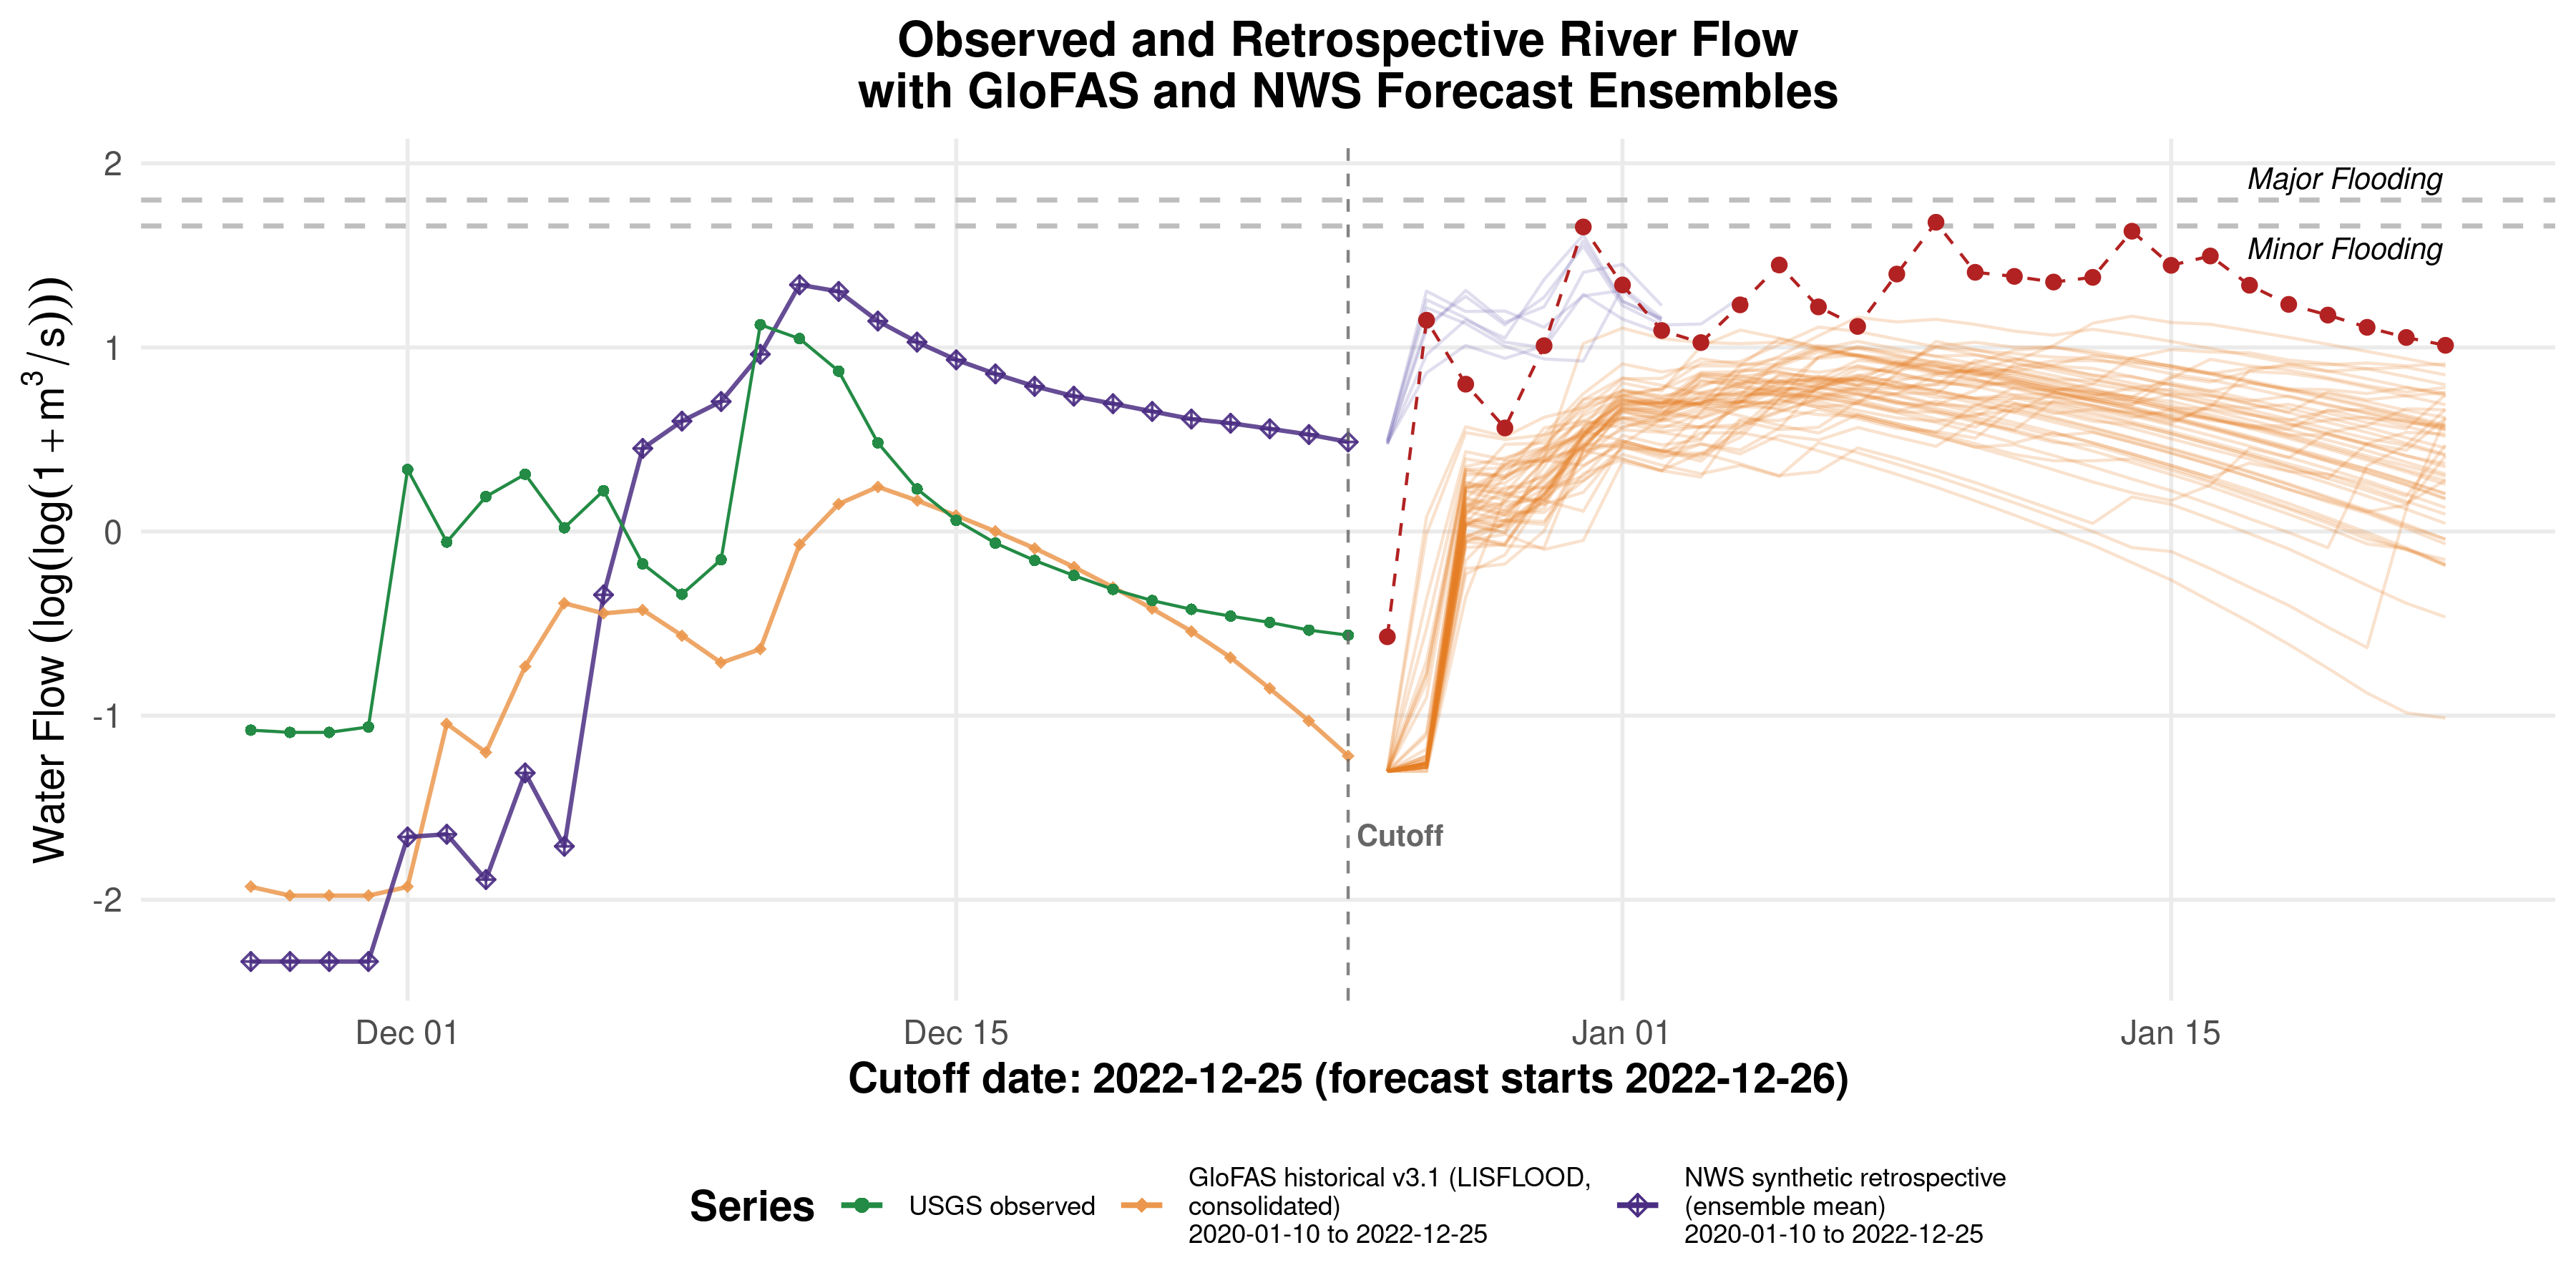
\includegraphics[width=450pt]{DISC/forecats.png}}
\caption{
\textbf{Before 2022-12-26:} Green—USGS observations; Purple—NWS retrospective analysis; Orange—GloFAS retrospective analysis. \textbf{From 2022-12-26 onward:} Red—future USGS observations used only for verification; Purple—NWS 7-member forecast product, covering 2022-12-25 to 2023-01-05; Orange—GloFAS 51-member forecast product, covering 2022-12-25 to 2023-01-22. Horizontal dashed lines indicate official flood stages for the river.
}
\label{fig:ensembles}
\end{figure*}

\section{FORECAST VALIDATION RESULTS}
\label{sec:forecastvalidation}

\subsection{Comparative Forecasting Performance Across Model Families}
\label{subsec:benchmarkresults}

We fit the framework separately at the seven target quantile levels \(0.05\), \(0.20\), \(0.35\), \(0.50\), \(0.65\), \(0.80\), and \(0.95\). Forecast skill is then evaluated over each forecast window by the mean continuous ranked probability score (CRPS), using the variational Bayes fits described in Section~\ref{subsec:prioranddisc}.

Table~\ref{tab:benchmark_crps_models} compares the raw forecast products with nine Bayesian variants of the common state-space framework. These variants differ only in three respects: the observation likelihood, whether the synthesis uses only the USGS series or the full multivariate data set, and whether the transfer component remains active during the forecast window. We summarize them with the label \(L\)-\(S\)-\(T\), where \(L\in\{\mathrm{N},\mathrm{AL},\mathrm{exAL}\}\) indexes the likelihood, \(S\in\{\mathrm{U},\mathrm{M}\}\) indicates univariate or multivariate synthesis, and \(T\in\{\mathrm{T0},\mathrm{T1}\}\) indicates whether the transfer component is inactive or active during the forecast window. The raw baselines are the daily GloFAS and NWM forecast products evaluated without statistical correction.

\begin{table*}[htbp]
\centering
\renewcommand{\arraystretch}{1.08}
\caption{Mean forecast-window CRPS by model family and cutoff across the five rolling-origin evaluation folds. Lower values are better; bold indicates the lowest CRPS within each cutoff column.}
\label{tab:benchmark_crps_models}
\begin{tabular*}{\textwidth}{@{\extracolsep{\fill}} >{\ttfamily}l r r r r r}
\toprule
Model label & 01/23/2021 & 11/12/2021 & 12/21/2021 & 05/11/2022 & 12/25/2022 \\
\midrule
\multicolumn{6}{l}{\textit{Raw forecast products}} \\
RAW-GLOFAS & 0.5379 & 1.5664 & 1.7757 & 2.0301 & 2.9297 \\
RAW-NWM & 2.6668 & 0.0968 & 1.8160 & 0.7329 & 1.6609 \\
\addlinespace[2pt]
\multicolumn{6}{l}{\textit{Bayesian models (simple to complex)}} \\
N-U-T1 & 0.5851 & 0.9105 & 1.1922 & 1.3156 & 1.1617 \\
N-M-T0 & 0.3599 & 0.3226 & 2.0461 & 0.9356 & 3.2322 \\
N-M-T1 & 4.4601 & 0.3557 & 1.8789 & 1.3256 & 2.8785 \\
AL-U-T1 & 0.2946 & 0.1333 & 1.1377 & 0.0465 & 1.0293 \\
AL-M-T0 & 0.3252 & 0.2547 & 0.6708 & 0.0460 & 2.1955 \\
AL-M-T1 & 0.1421 & 0.0237 & 0.3595 & 0.0223 & 0.6640 \\
exAL-U-T1 & 0.2969 & 0.1350 & 1.2043 & 0.0468 & 0.9324 \\
exAL-M-T0 & 0.3315 & 0.2836 & 0.5746 & 0.0695 & 2.2785 \\
exAL-M-T1 & \textbf{0.1295} & \textbf{0.0201} & \textbf{0.2830} & \textbf{0.0165} & \textbf{0.5991} \\
\bottomrule
\end{tabular*}
\end{table*}

Table~\ref{tab:benchmark_crps_models} yields a consistent ranking across the five cutoffs. The two multivariate specifications with an active forecast-window transfer component, AL-M-T1 and exAL-M-T1, dominate the comparison, with exAL-M-T1 attaining the lowest CRPS in every cutoff. AL-M-T1 is the closest competitor, especially at 01/23/2021 and 05/11/2022, but it remains second in each case. The best corrected model also improves on the best raw forecast-product baseline in all five cutoffs. These results show that forecast skill improves when retrospective products are synthesized jointly with the observations and when the transfer component remains active during the forecast window. We therefore use exAL-M-T1 as the reference specification for the remaining summaries.

\section{INTERPRETATION OF THE SELECTED SPECIFICATION}
\label{sec:interpretation}

Because exAL-M-T1 attains the lowest CRPS in all five rolling-origin cutoffs, the remaining discussion focuses on that specification. Detailed source-specific summaries for the exAL shape and scale parameters are reported in Appendix~\ref{app:sourceparams}. In the main text, we focus on the aspects of the selected model that are most informative for interpretation.

\subsection{Covariate Effects}

\begin{table*}[htbp]
\centering
\renewcommand{\arraystretch}{1.13}
\begin{threeparttable}
\caption{Posterior Means and 95\% Credible Intervals for Covariate Effects}
\label{tab:components_23_31}
\begin{tabular*}{\textwidth}{@{\extracolsep{\fill}} l c S[table-format=-1.3] l }
\toprule
\textbf{Covariate} & \textbf{Quantile} & \textbf{Mean} & \textbf{95\% CI} \\
\midrule
\multirow{3}{*}{Precipitation}
  & 5th  & 1.945 & $[1.917,\ 1.973]$ \\
  & 50th & 2.392 & $[2.354,\ 2.429]$ \\
  & 95th & 2.946 & $[2.913,\ 2.978]$ \\
\midrule
\multirow{3}{*}{Soil Moisture}
  & 5th  & 0.115 & $[0.110,\ 0.119]$ \\
  & 50th & 0.118 & $[0.113,\ 0.124]$ \\
  & 95th & 0.253 & $[0.247,\ 0.259]$ \\
\midrule
\multirow{3}{*}{1st Principal Component}
  & 5th  & -0.084 & $[-0.087,\ -0.080]$ \\
  & 50th & -0.063 & $[-0.067,\ -0.059]$ \\
  & 95th & -0.032 & $[-0.036,\ -0.028]$ \\
\bottomrule
\end{tabular*}
\begin{tablenotes}
\item \textit{Note:} Posterior means and 95\% credible intervals $[{\rm Q2.5}, {\rm Q97.5}]$ for covariate coefficients in the transfer function, at final time $T$, for the 5th, 50th, and 95th quantile models.
\end{tablenotes}
\end{threeparttable}
\end{table*}

Table~\ref{tab:components_23_31} reports posterior means and 95\% credible intervals for the transfer-function coefficients at the 5th, 50th, and 95th quantiles. Precipitation has the largest positive effect and increases with the quantile level, indicating that it is the dominant driver of upper-tail flow behavior. Soil moisture is also positive at all three quantiles, with a stronger effect in the upper tail, which is consistent with antecedent wetness amplifying runoff during storms.

The first principal component remains negative and comparatively small after conditioning on precipitation and soil moisture, so its role is secondary to the local hydrometeorological covariates. Taken together, these estimates indicate that the transfer component is driven primarily by precipitation and antecedent wetness, with the climate index acting as a broader large-scale adjustment.

\subsection{Historical Behavior Across Representative Regimes}

To illustrate how the selected specification adapts across contrasting hydrological conditions, we focus on the 5th, 50th, and 95th quantiles during the 2012--2016 drought and the 2017--2019 wet period.

\begin{figure}[h]
\centering
\includegraphics[width=450pt]{DISC/All_exal_2012-2016_DISC.png}
\caption{
Posterior mean and 95\% credible intervals of river flow quantiles during the dry period (2012--2016). Shown are estimates for the 5th (red), 50th (green), and 95th (blue) quantile models, along with observed daily USGS flow (black). Horizontal dashed lines mark NOAA-defined minor and major flooding thresholds.
}
\label{fig:dry_quantile}
\end{figure}

\begin{figure}[h]
\centering
\includegraphics[width=450pt]{DISC/All_exal_2017-2019_DISC.png}
\caption{
Posterior mean and 95\% credible intervals of river flow quantiles during the wet period (2017--2019). Shown are estimates for the 5th (red), 50th (green), and 95th (blue) quantile models, along with observed daily USGS flow (black). Horizontal dashed lines mark NOAA-defined minor and major flooding thresholds.
}
\label{fig:rainy_quantile}
\end{figure}

Figures~\ref{fig:dry_quantile} and \ref{fig:rainy_quantile} show clear differences between the drought and wet-regime periods. During 2012--2016, the posterior bands remain comparatively narrow and the upper tail rarely approaches the flood thresholds. During 2017--2019, the upper tail widens substantially during the main winter events, and the 95th quantile exceeds the major flood stage in 2017 and 2019.

The contrast between these periods is most visible in the spread between the 5th and 95th quantiles. That spread remains relatively tight under dry conditions but expands during wet-season peaks, indicating that the selected specification allocates greater predictive spread when hydrological variability increases.

\subsection{Synthesized Predictive Illustration}
\label{subsec:synthillustration}

Figure~\ref{fig:synth1} illustrates the synthesized predictive distribution for the December 25, 2022 cutoff. It is included as an operational illustration of how the fitted quantile-specific forecasts combine into one predictive distribution; the comparative forecast evaluation remains the primary empirical evidence of the paper.

\begin{figure}[h]
\centering
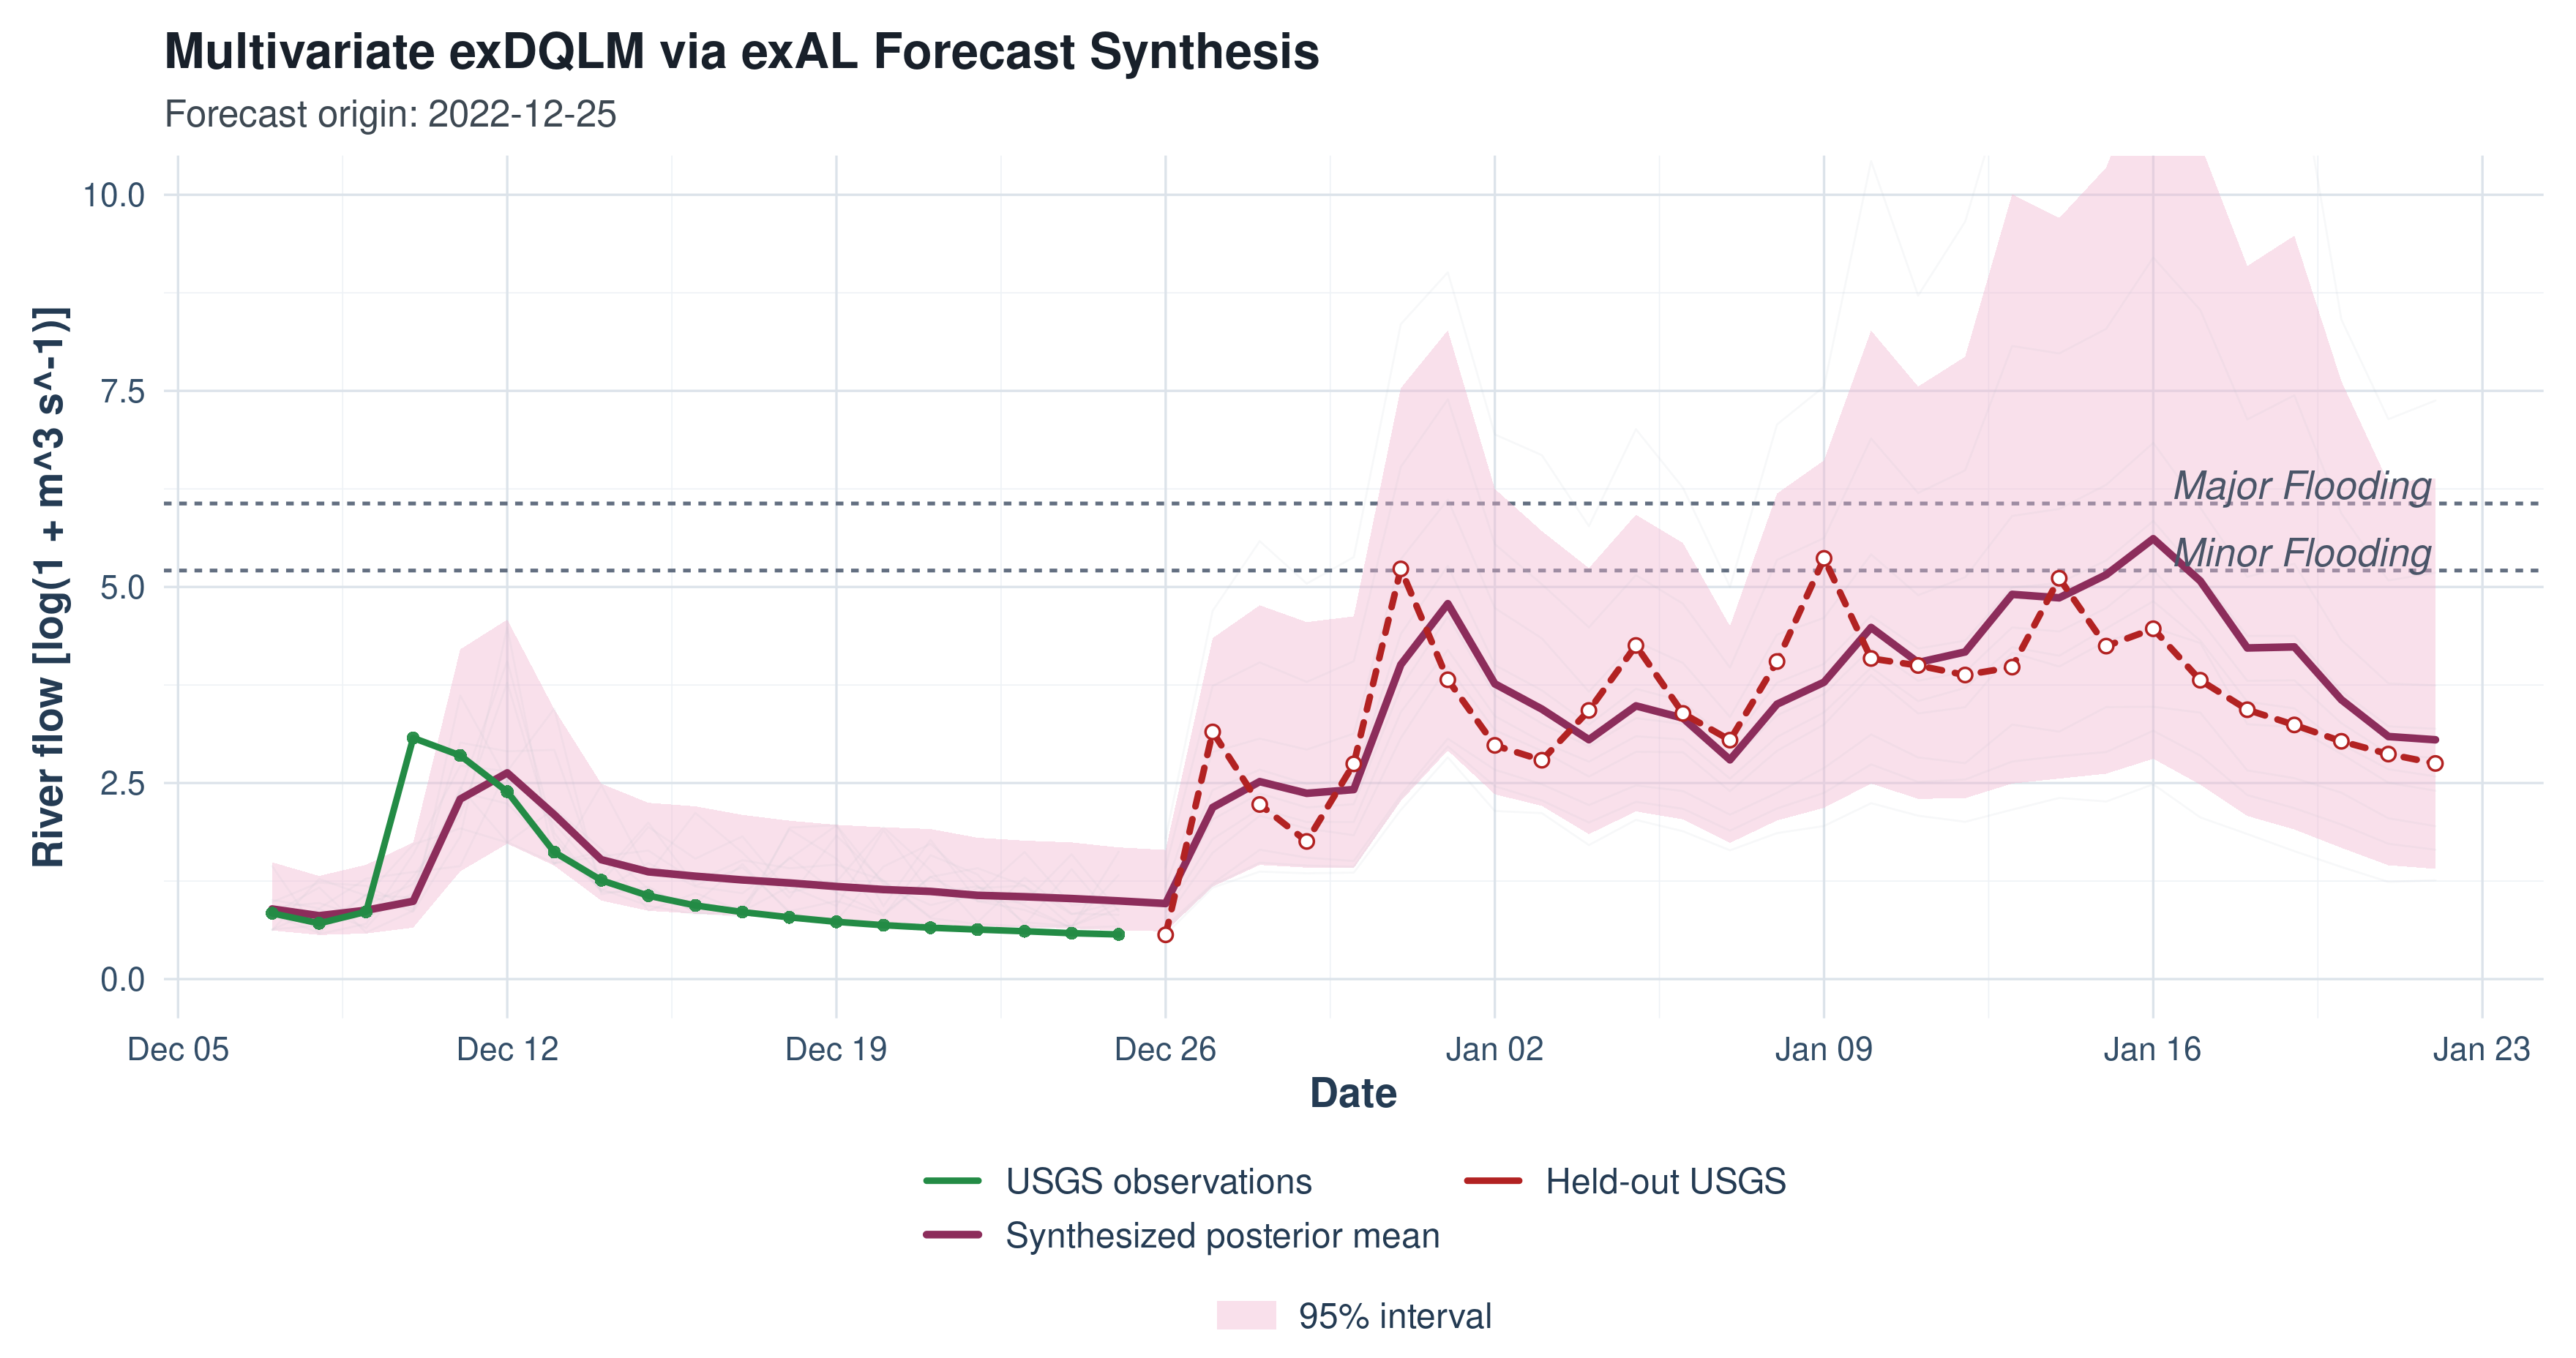
\includegraphics[width=450pt]{DISC/posterior_samples_valid.png}
\caption{
Synthesized posterior predictive distribution for river flow (log-log scale, cm$^3$/s) at the San Lorenzo River. Observed USGS measurements before December 25, 2022, are shown in green; unobserved future measurements are shown in red. Retrospective analyses (gray) are shown before December 25, and ensemble forecasts (gray) from ECMWF and NWS are shown after this date. Horizontal dashed lines indicate NOAA-defined minor and major flooding thresholds. The thin black lines shown along with the synthesized distribution (pink) correspond to the quantiles of the synthesized distribution (percentiles: 0.05, 0.20, 0.35, 0.5, 0.65, 0.8, 0.95). 
}
\label{fig:synth1}
\end{figure}
The synthesized predictive distribution combines observed USGS measurements before the cutoff with the retrospective and forecast products available at that origin. The upper quantiles rise sharply after December 25, 2022 and remain above the major flood threshold for several days, reflecting the high-risk character of this forecast window. An idealized historical-only reference is reported in Appendix~\ref{app:historicalsynth} to separate the operational synthesis from the simpler no-forecast counterfactual.

\section{Conclusions}
\label{sec5}

We developed a Bayesian quantile-based correction-and-synthesis framework for river-flow forecasting that links USGS observations, retrospective products, and forecast products through a shared latent quantile process. The framework combines source-specific discrepancy learning during the estimation period with a forecast-window extension that can propagate both retrospective corrections and transfer-component information into the prediction horizon. Variational Bayes based on Laplace--Delta approximations provides a scalable alternative to full MCMC for fitting the extended dynamic quantile linear model.

In the San Lorenzo application, the main empirical result is the five-cutoff rolling-origin forecast comparison based on the latest forecast products available at each cutoff. Relative to both simpler Bayesian variants and the raw forecast-product baselines, the multivariate specifications with an active forecast-window transfer component perform best, and exAL-M-T1 attains the lowest forecast-window CRPS in every case. These results indicate that forecast skill benefits from combining USGS observations with retrospective and forecast products, rather than treating each source in isolation.

The selected specification remains interpretable. The transfer component is driven primarily by precipitation and antecedent wetness, while the regime illustrations show that predictive spread widens during high-flow winter episodes and contracts during drought conditions. This combination of forecast performance and interpretability is important in applications where both uncertainty quantification and hydrological understanding matter.

The framework still depends on the quality and compatibility of the external products and on the availability of forecast covariates at each forecast origin. More broadly, its practical use in a new basin requires a version-consistent archive of observations, retrospective products, forecast products, and covariates. Natural extensions include joint treatment of multiple quantiles, richer dynamic structures for the discrepancy process, and spatial generalizations that couple nearby sites or basins.




\section*{Acknowledgments}

This work is part of the Ph.D. dissertation of Antonio Aguirre, as part of 
the program on statistical science at the University of
California Santa Cruz. The work was supported in part by the National Science
Foundation grant MMS2050012.

\section*{Code availability}

The reusable exDQLM estimation routines are available through the CRAN R package \texttt{exdqlm}. The end-to-end forecasting workflow used in this study is available at \url{https://github.com/AntonioAPDL/Project1}. Applying that workflow to a new basin still requires constructing a basin-specific, version-consistent archive of observations, retrospective products, forecast products, and forecast covariates.

%\subsection*{Author contributions}

%\subsection*{Financial disclosure}

%None reported.

%\subsection*{Conflict of interest}

%The authors declare no potential conflict of interests.

\clearpage


\appendix

\section{Additional Parameter and Illustrative Summaries}
\label{app:extras}

\subsection{Source-Specific Shape and Scale Parameters}
\label{app:sourceparams}

\begin{table*}[htbp]
\caption{Posterior Medians and 95\% Credible Intervals for $\gamma$ by Source and Quantile Level}
\label{tab:gamma_sigma_intervals1}
\centering
\renewcommand{\arraystretch}{1.08}
\begin{tabular*}{\textwidth}{@{\extracolsep{\fill}} l
  S[table-format=-1.3] l
  S[table-format=-1.3] l
  S[table-format=-1.3] l
  }
\toprule
\multirow{2}{*}{\textbf{Quantile}} &
\multicolumn{2}{c}{\textbf{USGS}} &
\multicolumn{2}{c}{\textbf{GLOFAS}} &
\multicolumn{2}{c}{\textbf{NWS}} \\
\cmidrule(lr){2-3} \cmidrule(lr){4-5} \cmidrule(lr){6-7}
& {\textbf{Median}} & {\textbf{95\% CI}}
& {\textbf{Median}} & {\textbf{95\% CI}}
& {\textbf{Median}} & {\textbf{95\% CI}} \\
\midrule
05th  & 0.796   & $[0.781,\ 0.809]$   & 1.06    & $[1.04,\ 1.07]$   & 0.991   & $[0.976,\ 1.01]$   \\
20th  & 0.0599  & $[0.0471,\ 0.0734]$ & 0.330   & $[0.318,\ 0.342]$ & 0.219   & $[0.206,\ 0.232]$ \\
35th  & -0.0232 & $[-0.0297,\ -0.0174]$ & 0.0827 & $[0.0739,\ 0.0911]$ & 0.0881 & $[0.0786,\ 0.0983]$ \\
50th  & -0.0997 & $[-0.109,\ -0.0906]$ & -0.0451 & $[-0.0517,\ -0.0382]$ & 0.00766 & $[-0.000356,\ 0.0146]$ \\
65th  & -0.285  & $[-0.297,\ -0.273]$ & -0.257  & $[-0.267,\ -0.248]$ & -0.0767 & $[-0.0870,\ -0.0671]$ \\
80th  & -0.655  & $[-0.673,\ -0.637]$ & -0.744  & $[-0.758,\ -0.731]$ & -0.212  & $[-0.224,\ -0.200]$ \\
95th  & -1.82   & $[-1.85,\ -1.80]$   & -2.38   & $[-2.41,\ -2.36]$   & -1.13   & $[-1.15,\ -1.12]$ \\
\bottomrule
\end{tabular*}
\begin{tablenotes}
\item \textit{Note:} Entries show the posterior median and the 95\% credible interval $[{\rm Q2.5}, {\rm Q97.5}]$ for each source and quantile.
\end{tablenotes}
\end{table*}

\begin{table*}[htbp]
\caption{Posterior Medians and 95\% Credible Intervals for $\sigma$ by Source and Quantile Level}
\label{tab:gamma_sigma_intervals2}
\centering
\renewcommand{\arraystretch}{1.08}
\begin{tabular*}{\textwidth}{@{\extracolsep{\fill}} l
  S[table-format=1.5] l
  S[table-format=1.5] l
  S[table-format=1.5] l
  }
\toprule
\multirow{2}{*}{\textbf{Quantile}} &
\multicolumn{2}{c}{\textbf{USGS}} &
\multicolumn{2}{c}{\textbf{GLOFAS}} &
\multicolumn{2}{c}{\textbf{NWS}} \\
\cmidrule(lr){2-3} \cmidrule(lr){4-5} \cmidrule(lr){6-7}
& {\textbf{Median}} & {\textbf{95\% CI}}
& {\textbf{Median}} & {\textbf{95\% CI}}
& {\textbf{Median}} & {\textbf{95\% CI}} \\
\midrule
05th  & 0.0281 & $[0.0277,\ 0.0285]$  & 0.0272 & $[0.0269,\ 0.0275]$  & 0.0332 & $[0.0327,\ 0.0336]$ \\
20th  & 0.0560 & $[0.0552,\ 0.0568]$  & 0.0563 & $[0.0556,\ 0.0570]$  & 0.0650 & $[0.0640,\ 0.0658]$ \\
35th  & 0.0745 & $[0.0734,\ 0.0755]$  & 0.0687 & $[0.0678,\ 0.0696]$  & 0.0813 & $[0.0802,\ 0.0824]$ \\
50th  & 0.0826 & $[0.0814,\ 0.0837]$  & 0.0743 & $[0.0734,\ 0.0753]$  & 0.0852 & $[0.0840,\ 0.0864]$ \\
65th  & 0.0817 & $[0.0805,\ 0.0828]$  & 0.0736 & $[0.0727,\ 0.0746]$  & 0.0805 & $[0.0794,\ 0.0816]$ \\
80th  & 0.0725 & $[0.0715,\ 0.0735]$  & 0.0677 & $[0.0668,\ 0.0685]$  & 0.0646 & $[0.0638,\ 0.0655]$ \\
95th  & 0.0435 & $[0.0429,\ 0.0440]$  & 0.0475 & $[0.0470,\ 0.0480]$  & 0.0356 & $[0.0351,\ 0.0361]$ \\
\bottomrule
\end{tabular*}
\begin{tablenotes}
\item \textit{Note:} Entries show the posterior median and the 95\% credible interval $[{\rm Q2.5}, {\rm Q97.5}]$ for each source and quantile.
\end{tablenotes}
\end{table*}

Tables~\ref{tab:gamma_sigma_intervals1} and \ref{tab:gamma_sigma_intervals2} summarize the source-specific skewness (\(\gamma\)) and scale (\(\sigma\)) parameters of the exAL observation model. The estimates vary across both source and quantile, which supports the use of source-specific exAL parameters rather than a single common shape-and-scale specification.

\subsection{Long-Cycle Seasonal Component}
\label{app:longcycle}

\begin{figure}[h]
\centering
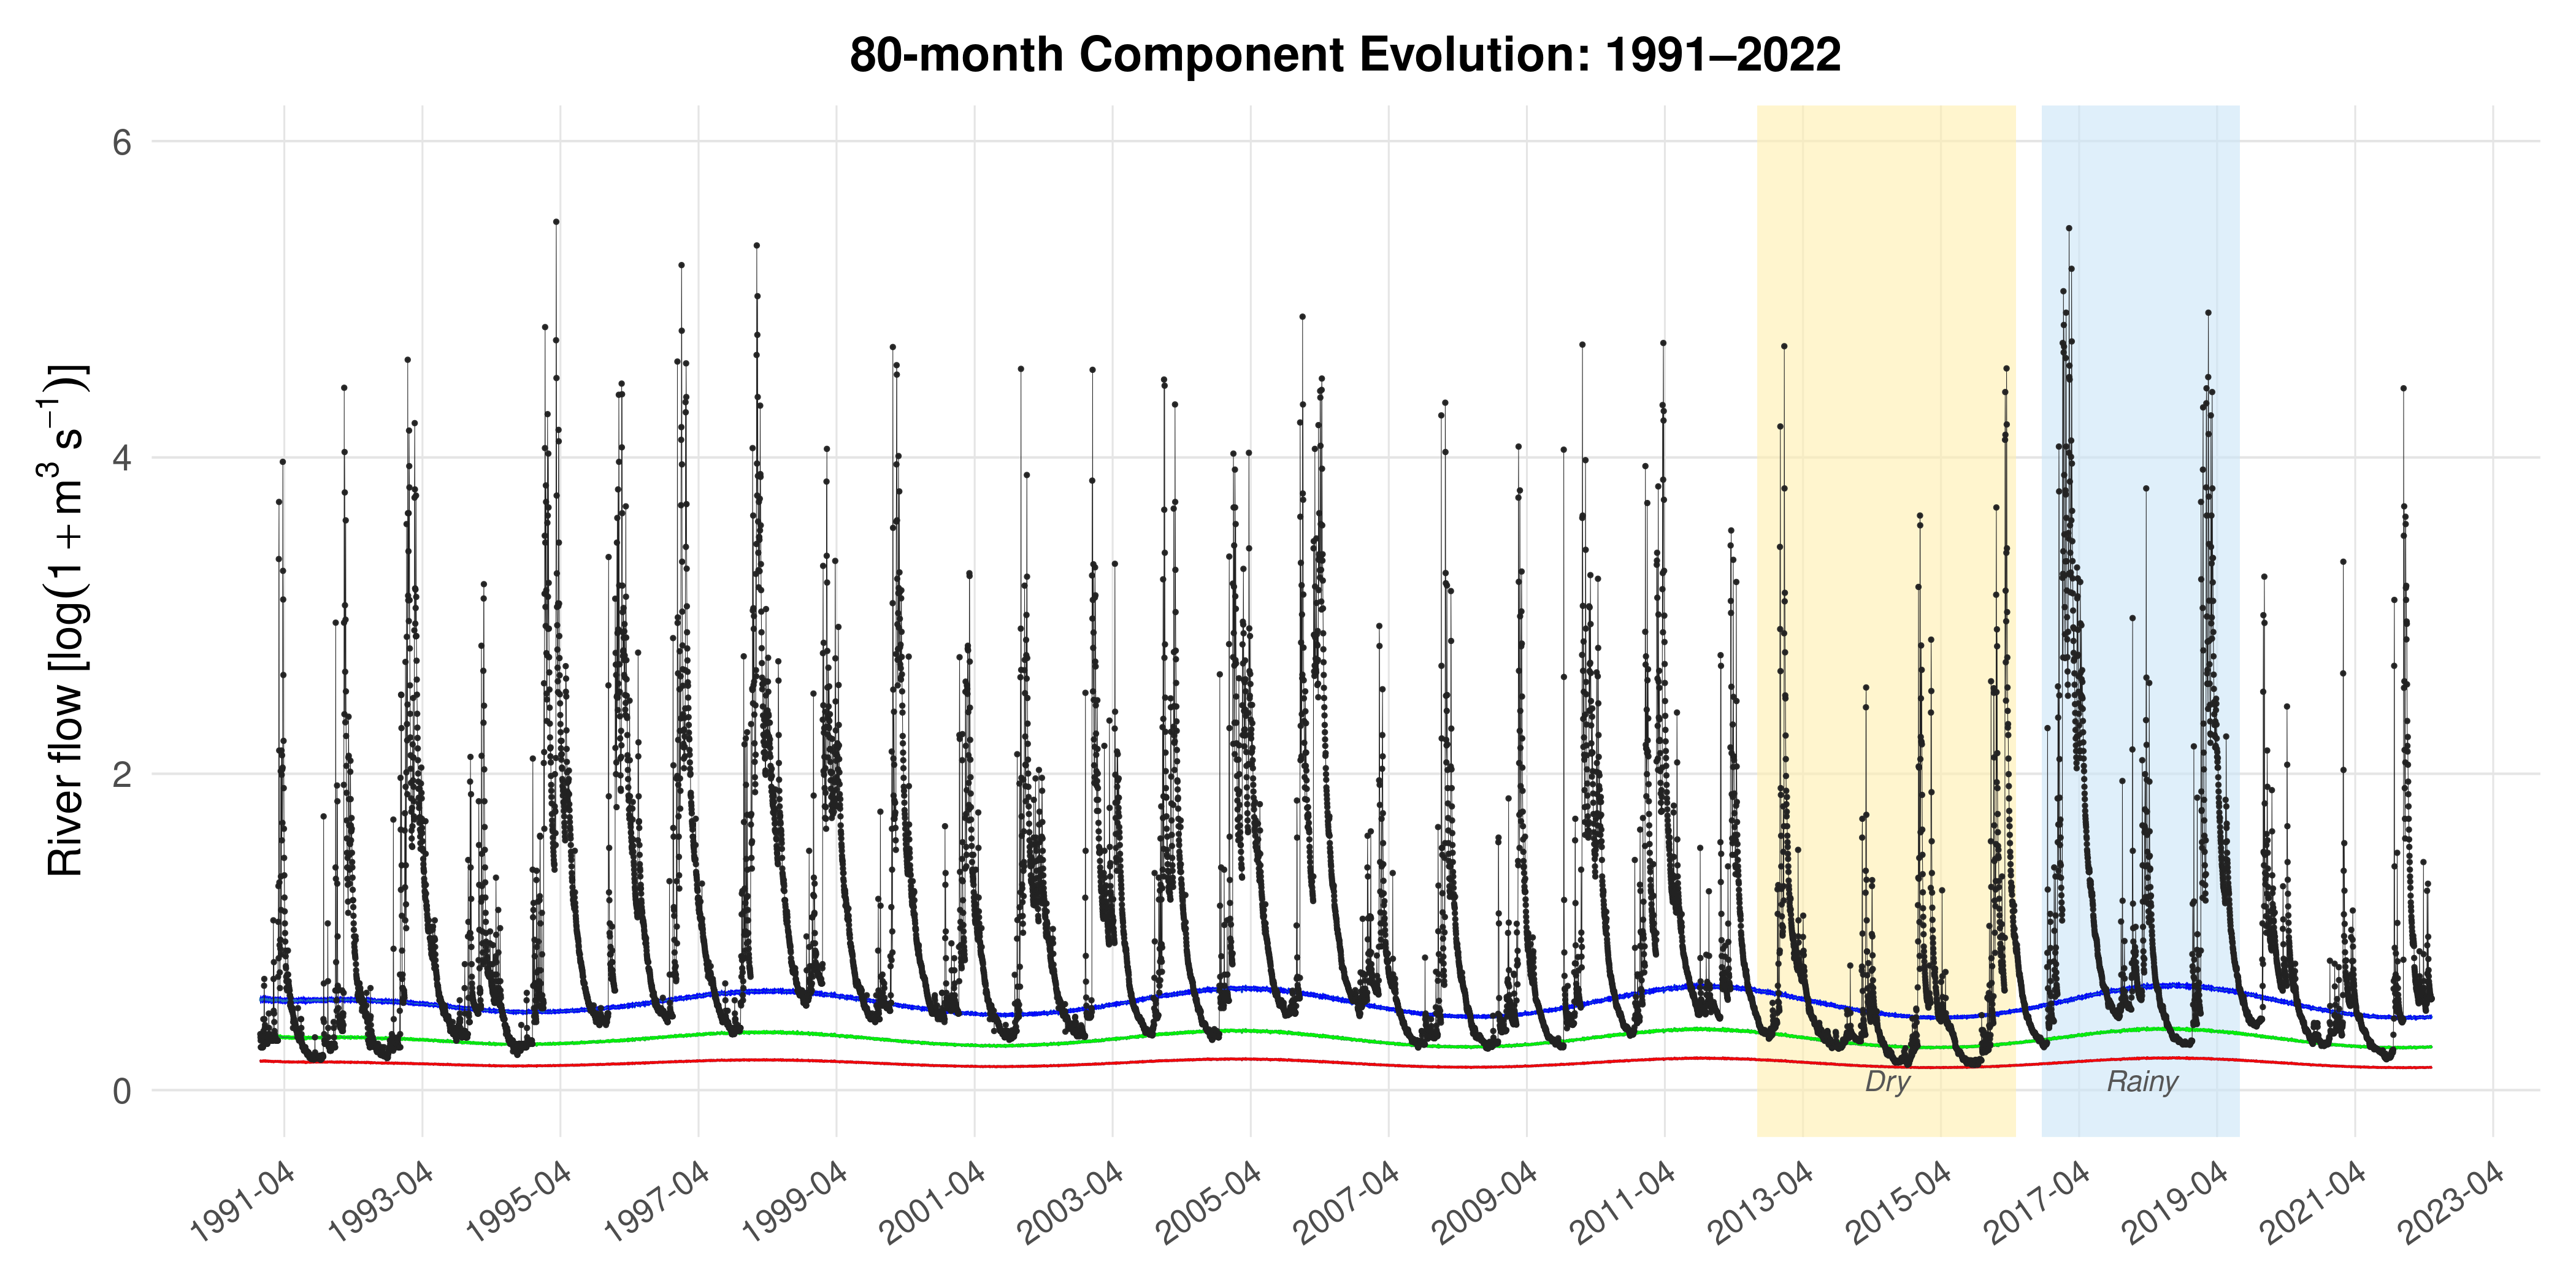
\includegraphics[width=450pt]{DISC/80_component_1991_2022.png}
\caption{
Posterior mean and 95\% credible intervals for the 80-month seasonal component of river flow from 1991 to 2022, estimated at the 5th (red), 50th (green), and 95th (blue) quantiles. Observed USGS daily flow is shown in black for reference.
}
\label{fig:80_components}
\end{figure}

Figure~\ref{fig:80_components} shows that the 80-month seasonal component is broadly aligned across the three representative quantiles and captures multi-year wet and dry phases in the historical record.

\subsection{Idealized Historical-Only Synthesis}
\label{app:historicalsynth}

\begin{figure}[h]
\centering
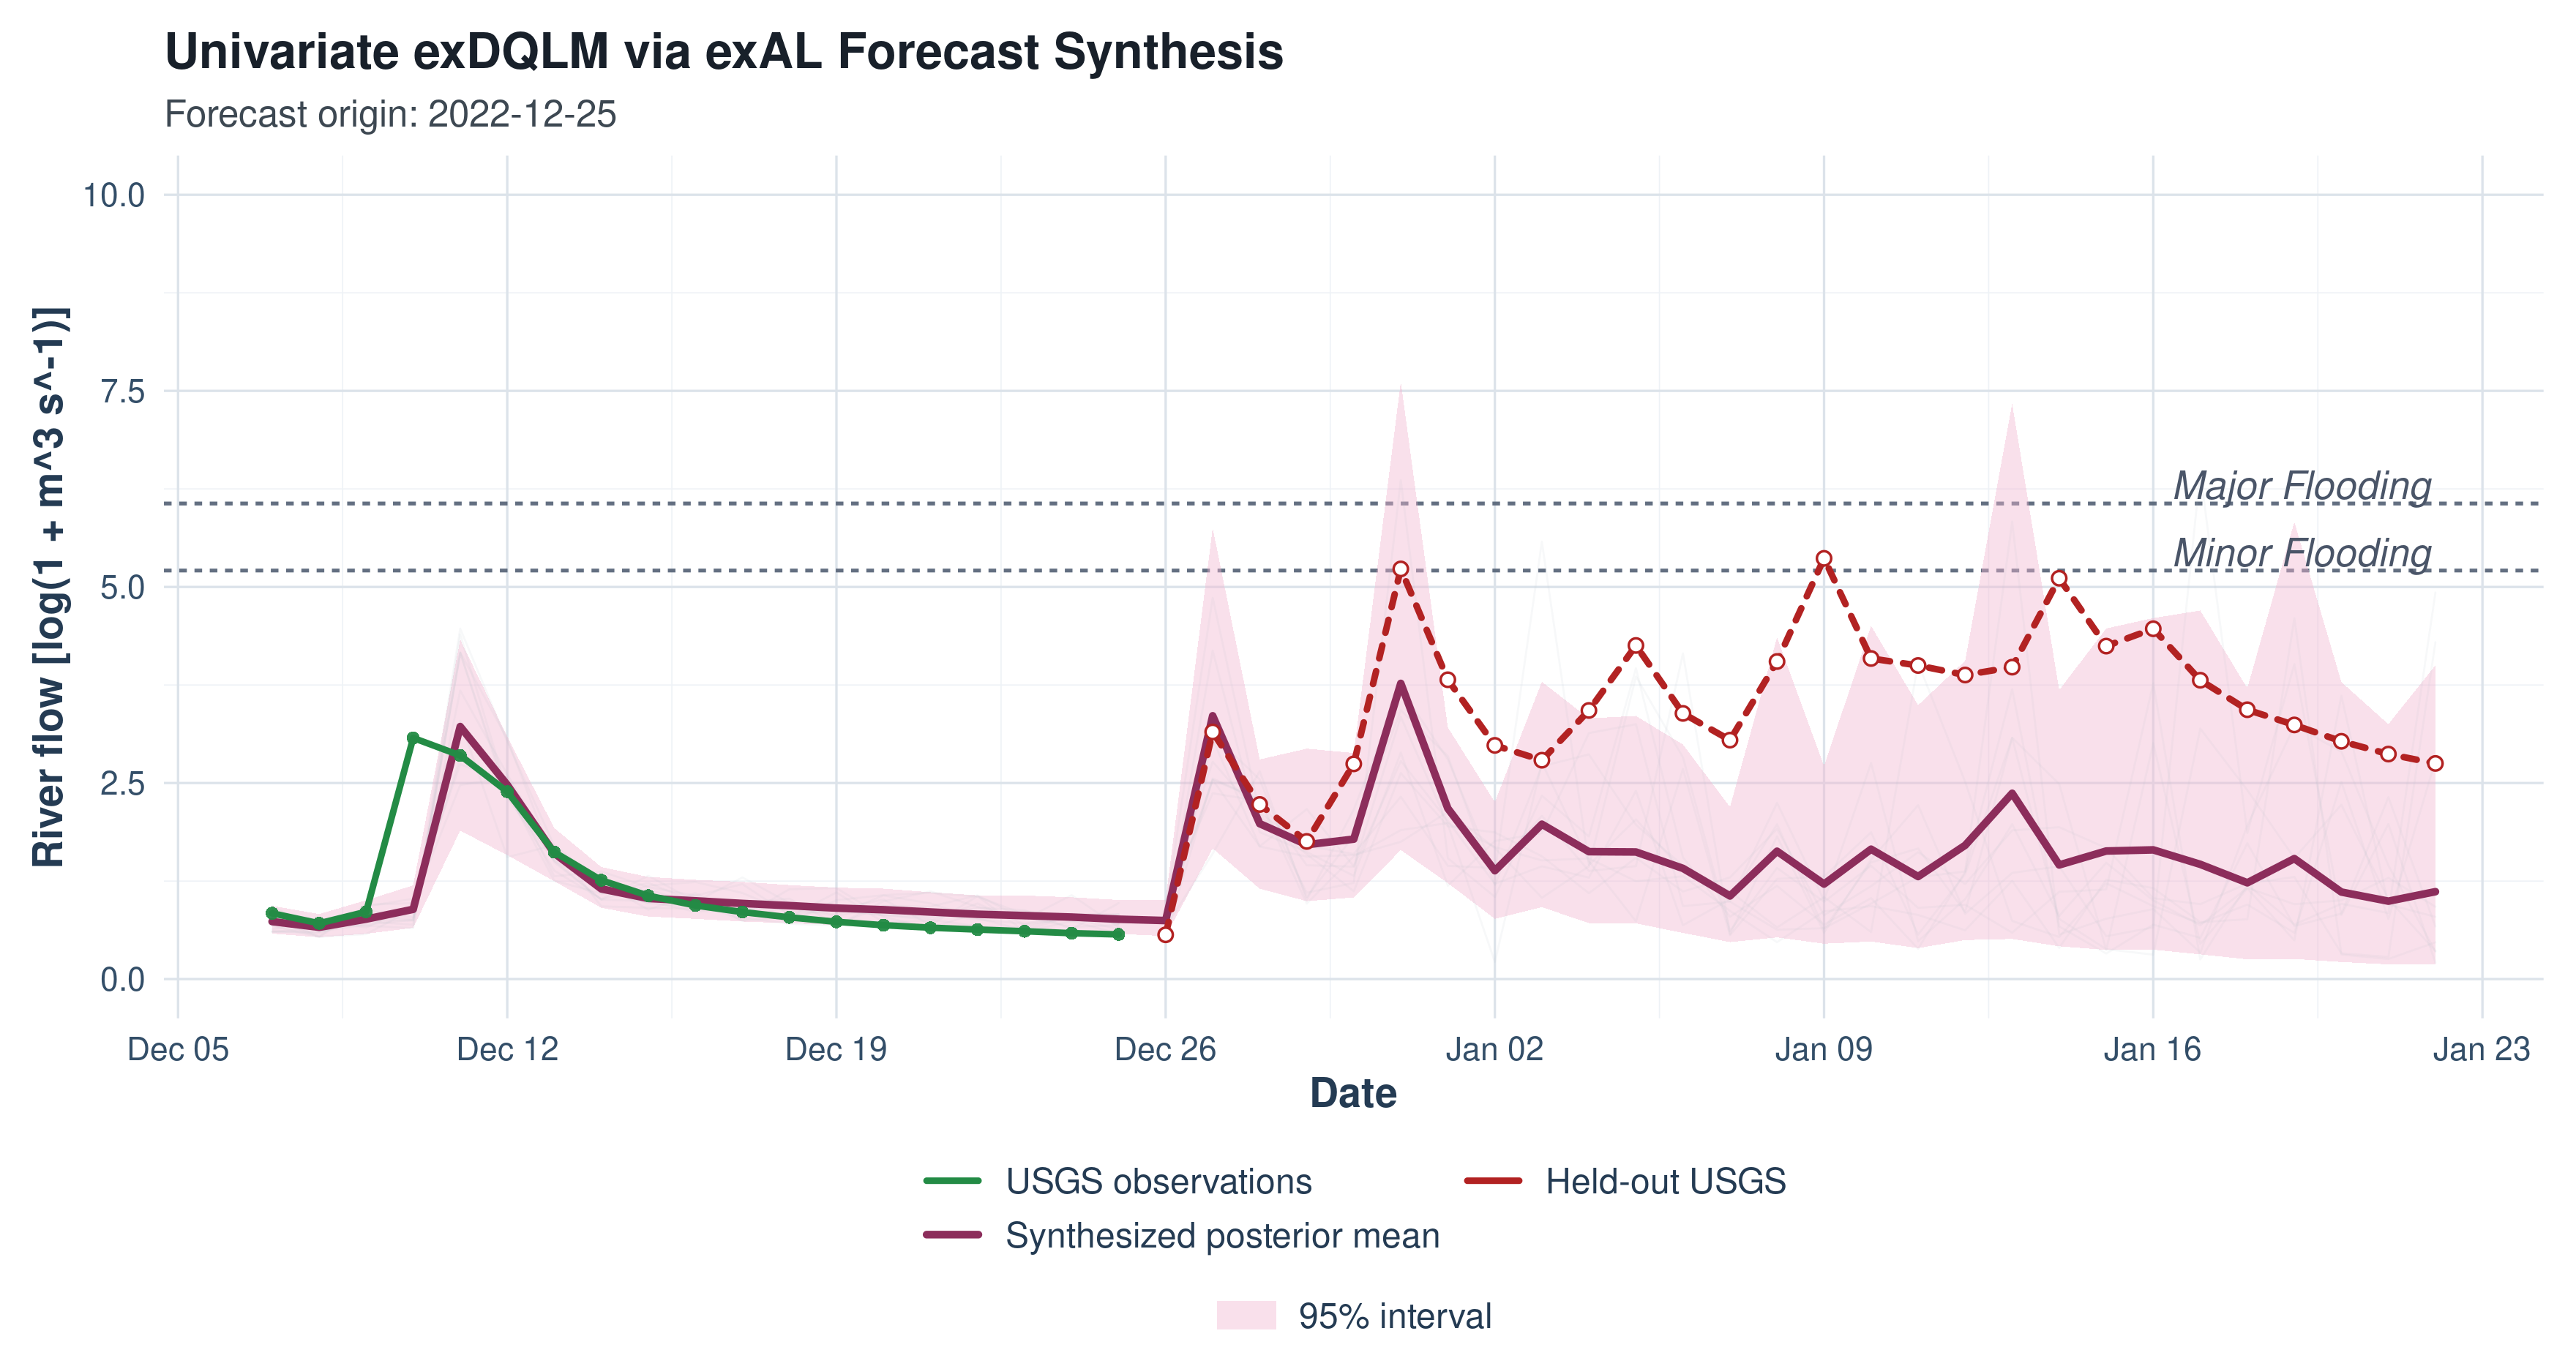
\includegraphics[width=450pt]{DISC/posterior_samples_counter_valid.png}
\caption{
Idealized benchmark synthesized posterior predictive distribution for river flow (log-log scale, cm$^3$/s), based only on historical observed USGS measurements. Observed measurements before December 25, 2022, are shown in green, and unobserved future measurements are shown in red. No retrospective analyses or ensemble forecasts are included. Horizontal dashed lines indicate NOAA-defined minor and major flooding thresholds. The thin black lines shown along with the synthesized distribution (pink) correspond to the quantiles of the synthesized distribution (percentiles: 0.05, 0.20, 0.35, 0.5, 0.65, 0.8, 0.95).
}
\label{fig:synth2}
\end{figure}

Figure~\ref{fig:synth2} provides a historical-only reference for the December 25, 2022 cutoff. It is included to contrast the operational synthesis in Figure~\ref{fig:synth1} with a simpler counterfactual that excludes retrospective and forecast products.

\section{Markov Chain Monte Carlo Algorithms}
\begin{algorithm}
\caption{MCMC Algorithm}\label{alg1}
\begin{algorithmic}

\State \textbf{Notation:}
\State  \(
A^j = A(\gamma^j;p_0), \quad B^j = B(\gamma^j;p_0), \quad C^j = C(\gamma^j;p_0), \text{ as defined in Section~\ref{subsec:exal}}
\)
\State For compactness, \(y_t^j\) denotes the active observation or product associated with source \(j\), and \(\mathbf{h}_{t,j}\) denotes the corresponding active selector vector.
\vspace{0.1cm}
\hline
\vspace{0.1cm}


\State \textbf{Step 0: Set initial values} and sample size $N$.
\State Initialize $\{ (v^j)^{(0)}_{1:T}$, $(s^j)^{(0)}_{1:T}$, $(\boldsymbol{\eta})^{(0)}_{1:T}, $(\sigma^j)^{(0)}$, $(\gamma^j)^{(0)}\}_{j=0}^J$
\For{$n = 1$ to $N$}
    \State \textbf{Step 1: Update $\boldsymbol{\eta}_t$}
    \State Use Algorithm~\ref{alg:Alg2}
    \For{$j = 0$ to $J$}
        \State \textbf{Step 2: Update $v^j_t$}
        \For{$t = 1$ to $T$}
            \State Sample $(v^j_t)^{(n)} \sim \mathcal{GIG}(a^j_t, b^j_t, c^j_t)$
            \State $a^j_t = \frac{1}{2}$
            \State $b^j_t = \frac{1}{(\sigma^j)^{(n-1)}}\left[ \frac{((A^j)^2)^{(n-1)}}{(B^j)^{(n-1)}}+2\right]$
            \State $c^j_t = \frac{1}{(\sigma^j)^{(n-1)} (B^j)^{(n-1)}}\left[y_t^j -\textbf{h}_{t,j}' \boldsymbol{\eta}^{(n)}_t -(C^j)^{(n-1)} (\sigma^j)^{(n-1)} |(\gamma^j)^{(n-1)}| (s^j_t)^{(n-1)} \right]^2$
        \EndFor
        \For{$t = T+1$ to $T+K_{(1)}$}
            \State Sample $(v^j_t)^{(n)} \sim \mathcal{GIG}(a^j_t, b^j_t, c^j_t)$
            \State $a^j_t = \frac{1}{2}$
            \State $b^j_t = \frac{1}{(\sigma^j)^{(n-1)}}\left[ \frac{((A^j)^2)^{(n-1)}}{(B^j)^{(n-1)}}+2\right]$
            \State $c^j_t = \frac{1}{(\sigma^j)^{(n-1)} (B^j)^{(n-1)}}\left[y_t^j -\textbf{h}_{t,j}' \boldsymbol{\eta}^{(n)}_t -(C^j)^{(n-1)} (\sigma^j)^{(n-1)} |(\gamma^j)^{(n-1)}| (s^j_t)^{(n-1)} \right]^2$
        \EndFor

        \State \textbf{Step 3: Update $s^j_t$}
        \For{$t = 1$ to $T$}
            \State Sample $(s^j)^{(n)}_t \sim \mathcal{N}^+(m^j_t, \lambda^j_t)$
            \State $\lambda^j_t =  \left[\frac{\big((C^j)^{(n-1)}\gamma^{(n-1)} \big)^2(\sigma^j)^{(n-1)}}{(B^j)^{(n-1)}(v^j_t)^{(n)}}+1\right]$
            \State $m^j_t =  \lambda^j_t \left[\frac{(C^j)^{(n-1)}|\gamma^{n-1}|(y_t^j -\textbf{h}_{t,j}' \boldsymbol{\eta}^{(n)}_t - (A^j)^{(n-1)} (v^j_t)^{(n)})}{(B^j)^{(n-1)}(v^j_t)^{(n)}}\right]$
        \EndFor

        \State \textbf{Step 4: Update $\sigma^j$}
        \State Sample $(\sigma^j)^{(n)} \sim \mathcal{GIG}(a^j_t, b^j_t, c^j_t)$
        \State $a^j_t = -(1.5T + a_{\sigma^j})$
        \State $b^j_t = \sum_{t=1}^T \frac{1}{(B^j)^{(n-1)} (v^j_t)^{(n)}} \left((C^j)^{(n-1)} |(\gamma^j)^{(n-1)}| (s^j_t)^{(n)} \right)^2$
        \State $c^j_t = \sum_{t=1}^T \frac{1}{(B^j)^{(n-1)} (v^j_t)^{(n)}}\big(y_t^j -\textbf{h}_{t,j}' \boldsymbol{\eta}^{(n)}_t - (A^j)^{(n-1)} (v^j_t)^{(n)}\big)^2 + 2 \sum_{t=1}^T  (v^j_t)^{(n)} + 2 b_{\sigma^j}$

        \State \textbf{Step 5: Update $\gamma^j$}
        \State Implement Metropolis-Hastings (MH)
    \EndFor
\EndFor

\end{algorithmic}
\end{algorithm}

\begin{algorithm}
\caption{MCMC - Forward Filtering Backward Sampling (FFBS)}
\label{alg:Alg2}
\begin{algorithmic}

\State \textbf{Notation:}
\State  $\mathbf{H}_t = [\mathbf{h}_{t,0}, \mathbf{h}_{t,1}, \ldots, \mathbf{h}_{t,J}]$, $\mathbf{Y}_t = [y_t^0, y_t^1, \ldots, y_t^J]'$, and $\mathbf{D}_t, \boldsymbol{\Lambda}_t$ are as defined in Subsection~\ref{subsec:fullmodel}
\State $\mathbf{M}_t= \mathbf{C} \odot  \mathbf{\sigma} \odot | \mathbf{\gamma} | \odot \mathbf{s}_t + \mathbf{A} \odot \mathbf{v}_t$, \quad $\mathbf{O}_t= \sqrt{\mathbf{B} \odot \mathbf{v}_t} \odot Diag
(\mathbf{\sigma}) \sqrt{\mathbf{B} \odot \mathbf{v}_t} \odot \mathbf{\sigma}$
\State  \(
\mathbf{A} = \big[ A(\gamma^j;p_0)   \big], \quad \mathbf{B} = \big[  B(\gamma^j;p_0)  \big], \quad \mathbf{C} = \big[ C(\gamma^j;p_0)   \big] \), \text{ as defined in Section~\ref{subsec:exal}}
\State \( \mathbf{v}_t = \big[  v^j_t   \big], \quad  \mathbf{s}_t = \big[ 
s^j_t  \big] , \quad \mathbf{\sigma} = \big[ \sigma^j  \big]
\)
\State \text{where } \odot \text{ is the Hadamard product}
\vspace{0.1cm}
\hline
\vspace{0.1cm}

\State \textbf{Step 1: Forward Filtering}
\For{$t = 1$ to $T$}
    \State Compute Prior moments:
    \State $\mathbf{a}_t = \mathbf{D}_t \mathbf{m}_{t-1}$
    \State $\mathbf{R}_t = \mathbf{D}_t \mathbf{C}_{t-1} \mathbf{D}_t' +  \boldsymbol{\Lambda}_t$

    \State One-step-ahead forecast:
    \State $\mathbf{f}_t = \mathbf{H}_t' \mathbf{a}_t + \mathbf{M}_t$
    \State $\mathbf{Q}_t = \mathbf{H}_t' \mathbf{R}_t \mathbf{H}_t + \mathbf{O}_t$
    
    \State Compute Posterior moments:
    \State $\mathbf{m}_t = \mathbf{a}_t + \mathbf{R}_t \mathbf{H}_t \mathbf{Q}_t^{-1}(\mathbf{Y}_t - \mathbf{f}_t)$
    \State $\mathbf{C}_t = \mathbf{R}_t - \mathbf{R}_t \mathbf{H}_t \mathbf{Q}_t^{-1} \mathbf{H}_t' \mathbf{R}_t$
\EndFor

\State \textbf{Step 2: Backward Sampling}
\For{$t = T$ down to $0$}
    \If{$t = T$}
        \State Sample $\boldsymbol{\eta}_T | D_T \sim \mathcal{N}(\mathbf{m}_T, \mathbf{C}_T)$
    \Else
        \State Compute Retrospective moments:
        \State $\mathbf{m}_t^s = \mathbf{m}_t + \mathbf{C}_t \mathbf{D}_{t+1}' \mathbf{R}_{t+1}^{-1} (\boldsymbol{\eta}_{t+1} - \mathbf{a}_{t+1})$
        \State $\mathbf{C}_t^s = \mathbf{C}_t - \mathbf{C}_t \mathbf{D}_{t+1}' \mathbf{R}_{t+1}^{-1} \mathbf{D}_{t+1} \mathbf{C}_t$
        
        \State Sample $\boldsymbol{\eta}_t | D_T \sim \mathcal{N}(\mathbf{m}_t^s, \mathbf{C}_t^s)$
    \EndIf
\EndFor

\end{algorithmic}
\end{algorithm}

 \clearpage


\section{Variational Bayes Algorithms}

\begin{algorithm}
\caption{Variational Bayes (VB) Algorithm}
\label{alg:Alg3}
\begin{algorithmic}

\State \textbf{Notation:}
\State  $\left\langle g(\xi) \right\rangle = \mathbb{E}_\xi\left[ g(\xi) \right]$
\State  \(
A^j = A(\gamma^j;p_0), \quad B^j = B(\gamma^j;p_0), \quad C^j = C(\gamma^j;p_0), \text{ as defined in Section~\ref{subsec:exal}}
\)
\vspace{0.1cm}
\hline
\vspace{0.1cm}

\State \textbf{Step 0: Set initial values}

\While{$\text{ELBO}_k > \text{tol}$}
    \State \textbf{Step 1: Update $r(\boldsymbol{\eta}_t)=\mathcal{N}(m^{(k)}_t,C^{(k)}_t)$}
    \State Use Algorithm~\ref{alg:Alg4}

    \For{$j = 0$ to $J$}
        \State \textbf{Step 2: Update $r(v^j_t)=\mathcal{GIG}(a_t^{j,(k)},b_t^{j,(k)},c_t^{j,(k)})$}
        \For{$t = 1$ to $T$}
            \State $a_t^{j,(k)} = \frac{1}{2}$
            \State $b_t^{j,(k)} = \left\langle \frac{A^2}{\sigma^j B^j} \right\rangle^{(k-1)} + 2 \left\langle \frac{1}{\sigma^j} \right\rangle^{(k-1)}$
            \State $c_t^{j,(k)} = \left\langle \frac{1}{\sigma^j B^j} \right\rangle^{(k-1)} \Big[ (y_t^j)^2 - 2y_t^j \left\langle  \mathbf{h}_{t,j} \boldsymbol{\eta}_t \right\rangle^{(k)} + \left\langle (  \mathbf{h}_{t,j} \boldsymbol{\eta}_t )^2 \right\rangle^{(k)} \Big]$
            \State $\quad \quad -2 \left\langle s^j_t \right\rangle^{(k-1)} \left\langle \frac{C^j|\gamma^j|}{B^j} \right\rangle^{(k-1)} \Big[ y_t^j - \left\langle  \mathbf{h}_{t,j} \boldsymbol{\eta}_t \right\rangle^{(k)} \Big]$
            \State $\quad \quad + \left\langle (s^j_t)^2 \right\rangle^{(k-1)} \left\langle \frac{(C^j)^2\sigma^j|\gamma^j|^2}{B^j} \right\rangle^{(k-1)}$
        \EndFor

        \State \textbf{Step 3: Update $r(s^j_t)=\mathcal{N}^+(\eta^{j,(k)},\lambda^{j,(k)})$}
        \For{$t = 1$ to $T$}
            \State $\lambda^{j,(k)} = \Big[ 1+\left\langle \frac{(C^j)^2 \sigma^j |(\gamma^j)|^2}{B^j} \right\rangle^{(k-1)} \left\langle \frac{1}{v^j_t} \right\rangle^{(k)} \Big]^{-1}$
            \State $\eta^{j,(k)} = \lambda^{j,(k)}  \Big[ \left\langle \frac{C^j |\gamma^j|}{B^j} \right\rangle^{(k-1)} \left\langle \frac{1}{v^j_t} \right\rangle^{(k)} \Big( y_t^j - \left\langle  \mathbf{h}_{t,j} \boldsymbol{\eta}_t \right\rangle^{(k)} \Big) - \left\langle \frac{C^j |\gamma^j| A^j}{B^j} \right\rangle^{(k-1)} \Big]$
        \EndFor

        \State \textbf{Step 4: Update $r(\gamma^j, \sigma^j )$}
        \State Approximate via VB-LD, as described in Section~\ref{subsec:postinf}
    \EndFor
\EndWhile

\end{algorithmic}
\end{algorithm}

\begin{algorithm}
\caption{VB-Filtering and VB-Smoothing}
\label{alg:Alg4}
\begin{algorithmic}

\State \textbf{Notation:}
\State $\left\langle g(\xi) \right\rangle = \mathbb{E}_\xi\left[ g(\xi) \right]$
\State  $\mathbf{H}_t = [\mathbf{h}_{t,0}, \mathbf{h}_{t,1}, \ldots, \mathbf{h}_{t,J}]$, $\mathbf{Y}_t = [y_t^0, y_t^1, \ldots, y_t^J]'$, and $\mathbf{D}_t, \boldsymbol{\Lambda}_t$ are as defined in Subsection~\ref{subsec:fullmodel}
\State $\mathbf{M}_t= \mathbf{C} \odot  \mathbf{\sigma} \odot | \mathbf{\gamma} | \odot \mathbf{s}_t + \mathbf{A} \odot \mathbf{v}_t$, \quad $\mathbf{O}_t= \sqrt{\mathbf{B} \odot \mathbf{v}_t} \odot Diag
(\mathbf{\sigma}) \sqrt{\mathbf{B} \odot \mathbf{v}_t} \odot \mathbf{\sigma}$
\State  \(
\mathbf{A} = \big[ \left\langle A(\gamma^j;p_0)  \right\rangle \big], \quad \mathbf{B} = \big[ \left\langle B(\gamma^j;p_0)  \right\rangle \big], \quad \mathbf{C} = \big[ \left\langle C(\gamma^j;p_0)  \right\rangle \big] \), \text{ as defined in Section~\ref{subsec:exal}}
\State \( \mathbf{v}_t = \big[ \left\langle v^j_t  \right\rangle \big], \quad  \mathbf{s}_t = \big[ \left\langle
s^j_t  \right\rangle \big] , \quad \mathbf{\sigma} = \big[ \left\langle \sigma^j  \right\rangle \big]
\)
\State \text{where } \odot \text{ is the Hadamard product}
\vspace{0.1cm}
\hline
\vspace{0.1cm}

\State \textbf{Step 1: Forward Filtering}
\For{$t = 1$ to $T$}
    \State Compute Prior moments:
    \State $\mathbf{a}_t = \mathbf{D}_t \mathbf{m}_{t-1}$
    \State $\mathbf{R}_t = \mathbf{D}_t \mathbf{C}_{t-1} \mathbf{D}_t' +  \boldsymbol{\Lambda}_t$

    \State One-step-ahead forecast:
    \State $\mathbf{f}_t = \mathbf{H}_t'\mathbf{a}_t + \mathbf{M}_t$
    \State $\mathbf{Q}_t = \mathbf{H}_t'\mathbf{R}_t\mathbf{H}_t + \mathbf{O}_t$
    
    \State Compute Posterior moments:
    \State $\mathbf{m}_t = \mathbf{a}_t + \mathbf{R}_t \mathbf{H}_t \mathbf{Q}_t^{-1}(\mathbf{Y}_t - \mathbf{f}_t)$
    \State $\mathbf{C}_t = \mathbf{R}_t - \mathbf{R}_t \mathbf{H}_t \mathbf{Q}_t^{-1} \mathbf{H}_t' \mathbf{R}_t$
\EndFor

\State \textbf{Step 2: Backward Smoothing}
\For{$t = T$ down to $1$}
    \If{$t = T$}
        \State Set $r^{(k+1)}(\boldsymbol{\eta}_T) := \mathcal{N}(\mathbf{m}_T^s, \mathbf{C}_T^s)$
        \State $\mathbf{m}_T^s = \mathbf{m}_T$
        \State $\mathbf{C}_T^s = \mathbf{C}_T$
    \Else
        \State Compute Smoothing moments:
        \State $r^{(k+1)}(\boldsymbol{\eta}_t) := \mathcal{N}(\mathbf{m}_t^s, \mathbf{C}_t^s)$
        \State $B_t = \mathbf{C}_t \mathbf{D}_{t+1}' \mathbf{R}_{t+1}^{-1}$
        \State $\mathbf{m}_t^s = \mathbf{m}_t + \mathbf{B}_t (\mathbf{m}_{t+1}^s - \mathbf{a}_{t+1})$
        \State $\mathbf{C}_t^s = \mathbf{C}_t + \mathbf{B}_t (\mathbf{C}_{t+1}^s - \mathbf{R}_{t+1}) \mathbf{B}_t'$
    \EndIf
\EndFor


\end{algorithmic}
\end{algorithm}


\nocite{*}% 

\clearpage

\bibliography{wileyNJD-APA}%

\section*{Author Biography}

\begin{biography}{
\includegraphics[width=60pt,height=70pt  ]{empty}}{\textbf{Author Name.} This is sample author biography text this is.}
\end{biography}

\end{document}
